\section{Lineare Funktionen}
\begin{LA}
    {Einstiegsfrage 1}{}
    Um zum Flughafen zu gelangen, planen Alice und Bob, ein Taxi zu mieten.
    Dazu erkundigen sie sich bei zwei verschiedenen Taxiunternehmen
    nach den Tarifen.

    Bei \emph{Max-Taxi} gibt es eine Grundgebühr von 5 CHF und für jeden
    gefahrenen Kilometer bezahlt man zusätzlich 3.50 CHF.

    Bei \emph{Prestige-Taxi} beträgt die Grundgebühr 10 CHF.
    Pro gefahrenen Kilometer werden dafür nur 3 CHF verlangt.

    \begin{enumerate}
        \item Geben Sie die Gleichung der beiden Funktionen
              \(M(s)\) und \(P(s)\) an, welche der zurückgelegten
              Strecke \(s\) (in Kilometer) den Fahrpreis für die beiden
              Unternehmen Max-Taxi und Prestige-Taxi zuordnet.

              \[
                  M(s)=\hspace{4cm}
              \]
              \[
                  P(s)=\hspace{4cm}
              \]

        \item Betrachten Sie nun die Graphen der beiden Funktionen
              \(M(s)\) und \(P(s)\).

              \begin{center}
                  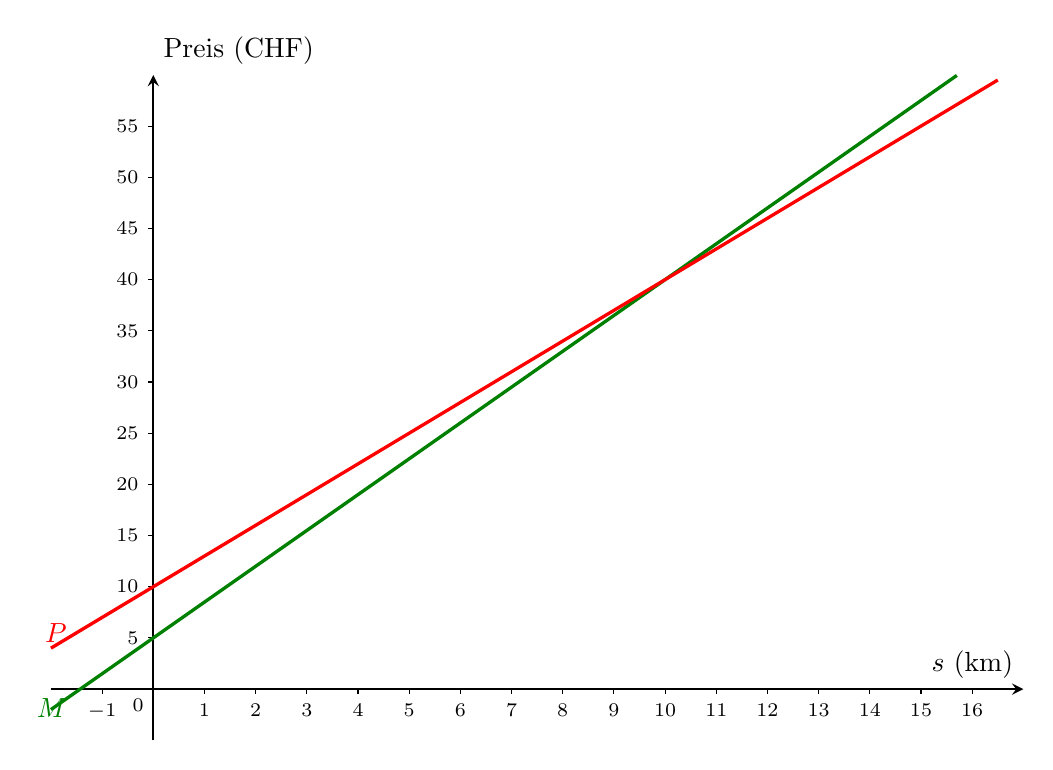
\begin{tikzpicture}[x=0.65cm,y=0.13cm,>=stealth]

                      % Achsen
                      \draw[->,thick] (-2,0) -- (17,0)
                      node[above left] {\(s\) (km)};

                      \draw[->,thick] (0,-5) -- (0,60)
                      node[above right] {Preis (CHF)};

                      % Beschriftung der s-Achse
                      \foreach \x in {1,...,16}
                      \draw (\x,0) -- (\x,-0.5)
                      node[below,font=\scriptsize] {\(\x\)};

                      \draw (-1,0) -- (-1,-0.5)
                      node[below,font=\scriptsize] {\(-1\)};

                      \node[below left,font=\scriptsize] at (0,0) {\(0\)};

                      % Beschriftung der Preisachse
                      \foreach \y in {5,10,...,55}
                      \draw (0,\y) -- (-0.1,\y)
                      node[left,font=\scriptsize] {\(\y\)};

                      % Max-Taxi
                      \draw[green!50!black,very thick,
                          domain=-2:15.7,samples=2]
                      plot (\x,{3.5*\x+5});

                      \node[green!50!black,below left]
                      at (-1.5,0) {\(M\)};

                      % Prestige-Taxi
                      \draw[red,very thick,
                          domain=-2:16.5,samples=2]
                      plot (\x,{3*\x+10});

                      \node[red,left]
                      at (-1.5,5.5) {\(P\)};

                  \end{tikzpicture}
              \end{center}

              \begin{enumerate}
                  \item Wie können am Graphen die Grundgebühren
                        der beiden Taxi-Unternehmen abgelesen werden?

                  \item Wie können am Graphen die Kosten pro Kilometer
                        der beiden Taxi-Unternehmen abgelesen werden?
              \end{enumerate}

        \item Wie kann man herausfinden, ab wie vielen Kilometern
              das eine Unternehmen günstiger als das andere ist?
              Kann man das nur graphisch herausfinden oder auch
              rechnerisch? Welcher Weg hat welche Vorteile?

        \item Bei den beiden Graphen handelt es sich um Geraden.
              Was könnte der Grund dafür sein?

    \end{enumerate}
\end{LA}

\clearpage
\begin{LA}
    {Wie steil ist die Gerade?}{}
    Alice hat die folgende Abbildung einiger Geraden vor sich.
    Sie ruft gleich Bob an, der die Grafik nicht sieht, und möchte
    ihm erzählen, wie die Geraden aussehen und insbesondere,
    wie steil sie sind.

    \begin{center}
        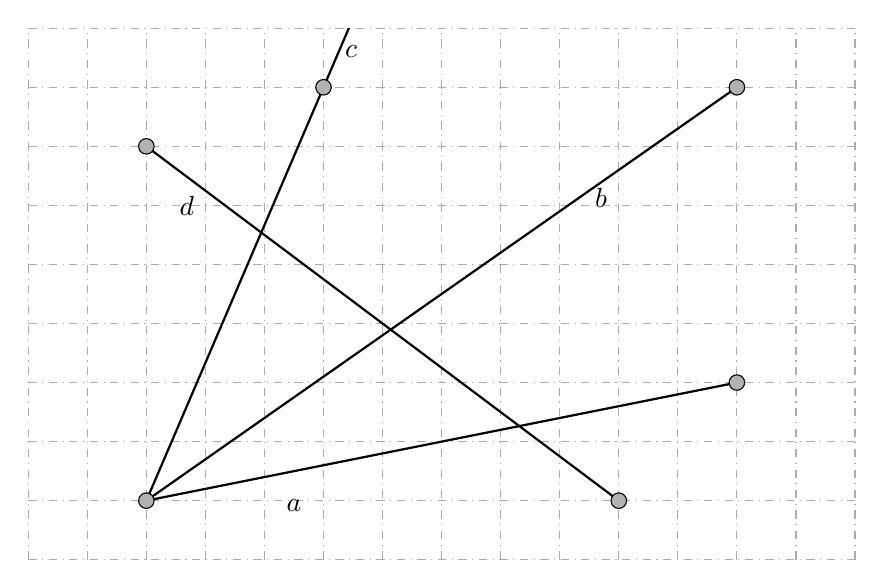
\begin{tikzpicture}[x=0.75cm,y=0.75cm]

            % Raster
            \draw[step=1,gray!65,dash dot]
            (0,0) grid (14,9);

            % Geraden
            \begin{scope}
                \clip (0,0) rectangle (14,9);

                % Gerade a: Steigung 1/5
                \draw[black,thick]
                (2,1) -- (12,3);

                % Gerade b: Steigung 7/10
                \draw[black,thick]
                (2,1) -- (12,8);

                % Gerade c: Steigung 7/3
                \draw[black,thick]
                (2,1) -- (5.5,9.1667);

                % Gerade d: Steigung -3/4
                \draw[black,thick]
                (2,7) -- (10,1);
            \end{scope}

            % Markierte Punkte
            \foreach \x/\y in {
                    2/1,
                    12/3,
                    12/8,
                    5/8,
                    2/7,
                    10/1
                } {
                    \filldraw[fill=gray!60,draw=black]
                    (\x,\y) circle (2.8pt);
                }

            % Beschriftungen
            \node[above] at (4.5,0.65) {\(a\)};
            \node[below] at (9.7,6.45) {\(b\)};
            \node[right] at (5.2,8.6) {\(c\)};
            \node[right] at (2.4,6.) {\(d\)};

        \end{tikzpicture}
    \end{center}

    \begin{center}
        \fbox{%
            \parbox{0.9\textwidth}{%
                \centering
                \Large Erfinden Sie eine Masszahl für
                \enquote{Steilheit}!
            }%
        }
    \end{center}

    Können Sie Alice bei diesem Unterfangen helfen?
    Genauer: Können Sie die Steilheit einer Geraden durch eine
    einzige Zahl ausdrücken, die Alice dann am Telefon nennen kann?

    Die Masszahl für Steilheit soll folgenden Regeln genügen:

    \begin{enumerate}
        \item Die Zahl soll für jede mögliche Gerade nach derselben
              Regel zustande kommen.

        \item Je grösser die Zahl ist, desto steiler ist die Gerade.
              (Die Grösse der Zahl gibt Bob also eine präzise Vorstellung
              davon, wie steil die Gerade ist.)

        \item Positive Zahlen stehen für Geraden, die streng monoton
              wachsen (wie a, b, c), und negative Zahlen stehen für Geraden,
              die streng monoton fallen (wie d).

        \item Es muss für Alice möglich sein, die Masszahlen für
              die Geraden a--d allein aus der abgebildeten Grafik
              ohne weitere Hilfsmittel präzise zu bestimmen.
    \end{enumerate}
\end{LA}











\clearpage
\subsection{Was ist eine lineare Funktion?}
In den ersten drei Kapiteln haben Sie gelernt, was Funktionen sind,
wie man sie graphisch darstellen kann und welche Eigenschaften des
Graphen häufig von Bedeutung sind. Im Folgenden werden Funktionen
untersucht, die in der Praxis häufig zur Anwendung kommen.
Dabei wird eine ähnliche Strategie wie bei den Gleichungen verfolgt:
Funktionen werden nicht einzeln untersucht, sondern gewissen Typen
zugeordnet, deren gemeinsamen Eigenschaften festgehalten werden.
Begonnen wird mit dem einfachsten Funktionstyp:
den \textbf{linearen Funktionen}.

\begin{definition}
    {Lineare Funktion}{}
    Eine Funktion mit einer Funktionsgleichung der Form
    \[
        f(x)=ax+b,
    \]
    heisst \textbf{lineare Funktion} oder
    \textbf{(Polynom-)Funktion 1. Grades}.
\end{definition}
\begin{bsp}
    {Linear oder nicht?}{}
    \begin{enumerate}
        \item Die Funktion \(f(x)=3x+1\) ist eine lineare Funktion
              (\(a=3,\ b=1\)).

        \item Die Funktion \(g(x)=-5+\frac{x}{3}\) ist eine lineare
              Funktion, denn sie ist von der Form
              \[
                  g(x)=\frac{1}{3}\cdot x+(-5)
              \]
              (\(a=\frac{1}{3},\ b=-5\)).

        \item Die Funktion \(h(x)=x\) ist eine lineare Funktion
              (\(a=1,\ b=0\)).

        \item Bei einer Funktion wie \(k(x)=3\) ist sich die
              Gemeinschaft der Mathematiker*innen nicht einig, ob sie
              zu den linearen Funktionen zählen soll. Die einen sagen ja
              (\(a=0,\ b=3\)), die anderen sagen, dass \(a=0\) nicht
              zulässig ist.

              Der Einfachheit halber werden wir sie als lineare Funktion
              betrachten.

        \item Die Funktionen \(y=x^2\), \(y=\frac{1}{x}\),
              \(y=\sqrt{x}\), \(y=10^x\) sind allesamt
              \textbf{keine} linearen Funktionen.
    \end{enumerate}
\end{bsp}

\textbf{Bemerkung}: Die Parameter \(a\) und \(b\) werden häufig auch mit \(m\) und \(q\) bezeichnet.

Als nächstes soll argumentiert werden, dass die Graphen von
linearen Funktionen stets Geraden sind. Zu diesem Zweck wird
untersucht, wie steil die Verbindungsstrecken zwischen zwei
Graphenpunkten sind. Wenn diese überall gleich steil verlaufen,
handelt es sich beim Graphen um eine Gerade.

\begin{center}
    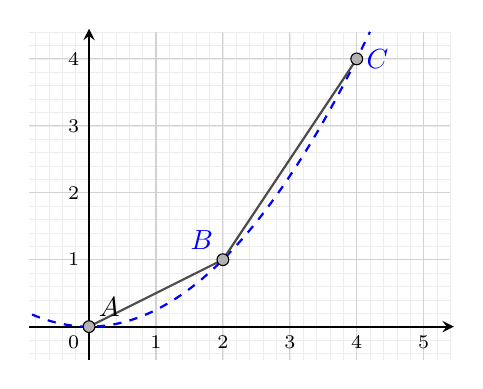
\begin{tikzpicture}[scale=0.85,>=stealth]

        % Feines Raster
        \draw[xstep=0.2,ystep=0.2,gray!15,very thin]
        (-0.9,-0.5) grid (5.4,4.4);

        % Hauptlinien
        \foreach \x in {0,...,5}
        \draw[gray!35,thin]
        (\x,-0.5) -- (\x,4.4);

        \foreach \y in {0,...,4}
        \draw[gray!35,thin]
        (-0.9,\y) -- (5.4,\y);

        % Achsen
        \draw[->,thick] (-0.9,0) -- (5.45,0);
        \draw[->,thick] (0,-0.5) -- (0,4.45);

        % Achsenbeschriftung
        \foreach \x in {1,...,5}
        \node[below,font=\scriptsize]
        at (\x,0) {\(\x\)};

        \node[below left,font=\scriptsize]
        at (0,0) {\(0\)};

        \foreach \y in {1,...,4}
        \node[left,font=\scriptsize]
        at (0,\y) {\(\y\)};

        % Funktionsgraph
        \draw[blue,dashed,thick,
            domain=-0.85:4.2,samples=201,smooth]
        plot (\x,{0.25*\x*\x});

        % Verbindungsstrecken
        \draw[black!70,thick]
        (0,0) -- (2,1) -- (4,4);

        % Punkte
        \filldraw[fill=gray!60,draw=black]
        (0,0) circle (2.5pt)
        (2,1) circle (2.5pt)
        (4,4) circle (2.5pt);

        % Punktbeschriftungen
        \node[above right] at (0,0) {\(A\)};
        \node[above left,blue] at (2,1) {\(B\)};
        \node[right,blue] at (4,4) {\(C\)};

    \end{tikzpicture}
\end{center}

Diese Idee versteht man vielleicht besser, wenn man ein
Beispiel eines Graphen betrachtet, der keine Gerade ist.
Weil die Strecke zwischen den Graphenpunkten \(AB\) weniger
steil verläuft als jene zwischen den Graphenpunkten \(BC\),
ist der Graph keine Gerade.

Damit die \enquote{Steilheit} zweier Strecken verglichen
werden kann, wird eine Masszahl dafür benötigt.










\clearpage
\subsection{Steigung einer Geraden}
\begin{center}
    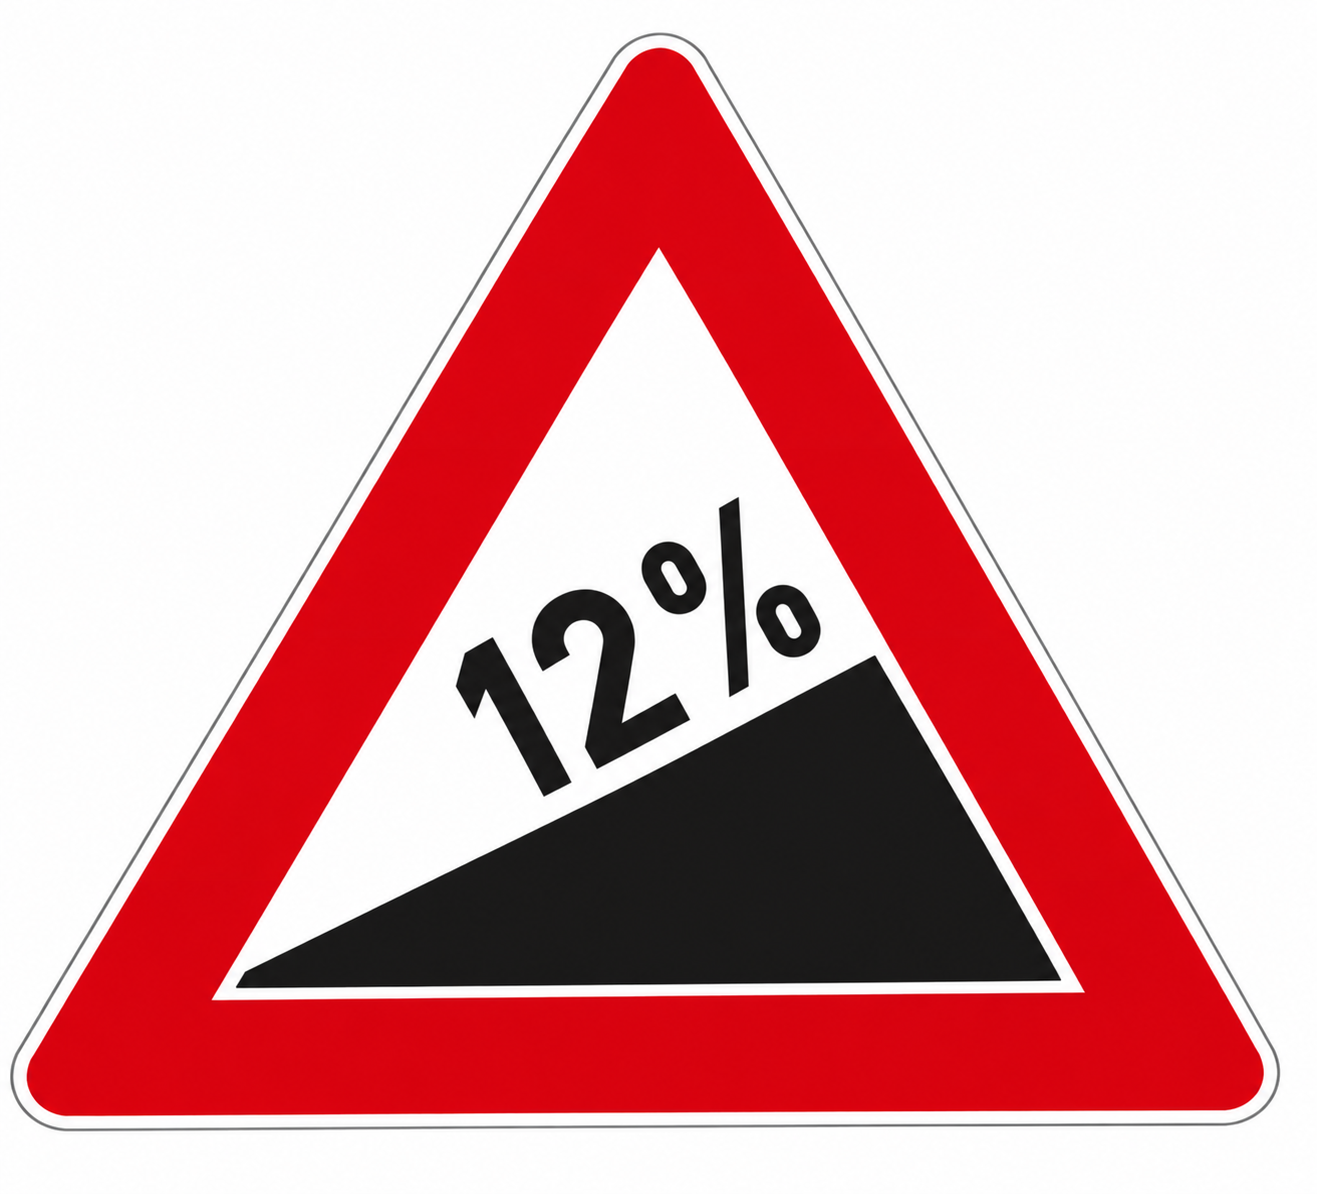
\includegraphics[width = 0.25\textwidth]{media/Verkehrszeichen_Steigung.png}
\end{center}
Hat eine Strasse eine Steigung von \(12\,\%\) bzw. \(0.12\),
bedeutet das, dass die Strasse auf 100 Meter in horizontaler
Richtung 12 Meter in vertikaler Richtung ansteigt.

Auf 50 Meter in horizontaler Richtung steigt die Strasse
entsprechend um \(0.12\cdot 50=6\) Meter an.
Auf 42 Meter in horizontaler Richtung beträgt der Anstieg
\(0.12\cdot 42=5.04\) Meter.

Die Steigung von \(12\,\%=0.12\) ist also das Verhältnis
des Anstiegs zur Strecke in horizontaler Richtung.

Genauso wird auch die Steigung einer Geraden im
Koordinatensystem definiert.

\begin{definition}
    {Steigung einer Geraden}{}
    Sei \(g\) eine Gerade im Koordinatensystem durch die Punkte
    \(A=(x_A, y_A)\) und \(B=(x_B, y_B)\).
    Die \textbf{Steigung} der Geraden \(g\) ist definiert als das Verhältnis
    \[
        \frac{\Delta y}{\Delta x}
        = \frac{y_B-y_A}{x_B-x_A}.
    \]

    \begin{center}
        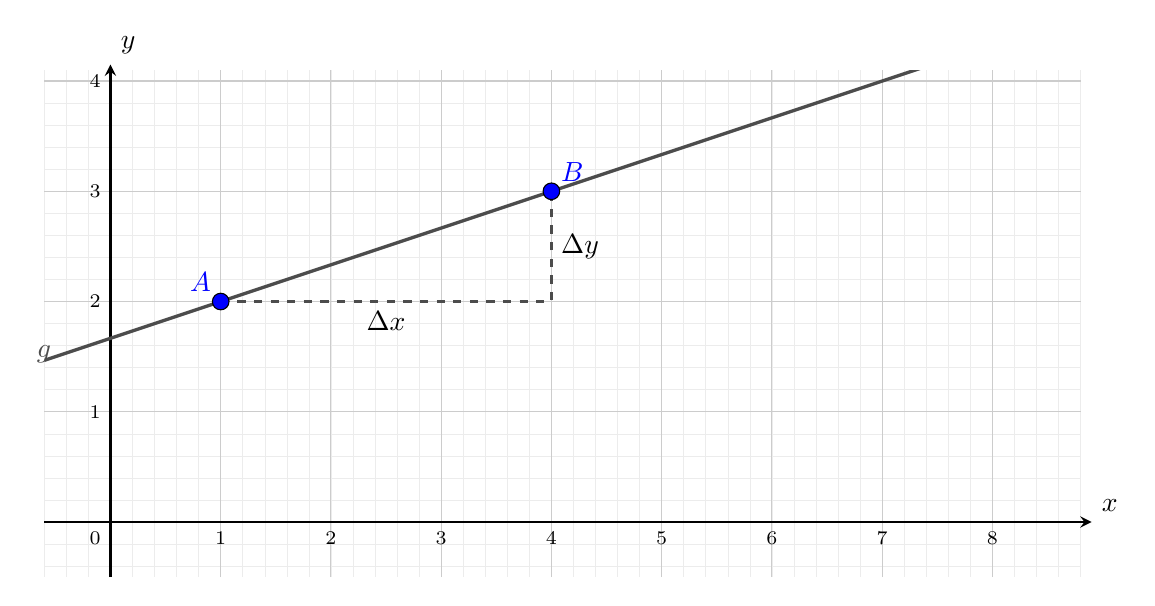
\begin{tikzpicture}[x=1.4cm,y=1.4cm,>=stealth]

            % Feines Raster
            \draw[xstep=0.2,ystep=0.2,gray!15,very thin]
            (-0.6,-0.5) grid (8.8,4.1);

            % Hauptlinien
            \foreach \x in {0,...,8}
            \draw[gray!40,thin]
            (\x,-0.5) -- (\x,4.1);

            \foreach \y in {0,...,4}
            \draw[gray!40,thin]
            (-0.6,\y) -- (8.8,\y);

            % Achsen
            \draw[->,thick] (-0.6,0) -- (8.9,0)
            node[above right] {\(x\)};
            \draw[->,thick] (0,-0.5) -- (0,4.15)
            node[above right] {\(y\)};
            % Achsenbeschriftung
            \foreach \x in {1,...,8}
            \node[below,font=\scriptsize]
            at (\x,0) {\(\x\)};

            \node[below left,font=\scriptsize]
            at (0,0) {\(0\)};

            \foreach \y in {1,2,3,4}
            \node[left,font=\scriptsize]
            at (0,\y) {\(\y\)};

            % Gerade g durch A(1|2) und B(4|3)
            \begin{scope}
                \clip (-0.6,-0.5) rectangle (8.8,4.1);
                \draw[black!70,very thick]
                (-0.6,{2+(-0.6-1)/3}) --
                (8.8,{2+(8.8-1)/3});
            \end{scope}

            \node[black!70,left] at (-0.45,1.52) {\(g\)};

            % Steigungsdreieck
            \draw[black!70,thick,dashed]
            (1,2) -- (4,2) -- (4,3);

            % Punkte A und B
            \filldraw[blue,draw=black]
            (1,2) circle (3pt)
            (4,3) circle (3pt);

            % Punktbeschriftungen
            \node[blue,above left] at (1,2) {\(A\)};
            \node[blue,above right] at (4,3) {\(B\)};

            % Beschriftung des Steigungsdreiecks
            \node[below] at (2.5,2) {\(\Delta x\)};
            \node[right] at (4,2.5) {\(\Delta y\)};

        \end{tikzpicture}
    \end{center}
\end{definition}
\clearpage
\textbf{Bemerkungen}

\begin{itemize}
    \item Das Symbol \(\Delta\) ist der griechische Grossbuchstabe
          \enquote{Delta} und steht für \enquote{Differenz}.
          Die Steigung ist das Verhältnis der Differenz der
          \(y\)-Koordinaten zur Differenz der \(x\)-Koordinaten.

    \item Die Gerade im Bild oben hat die Steigung
          \[
              \frac{\Delta y}{\Delta x}
              = \frac{3-2}{4-1}
              = \frac13.
          \]

    \item Es spielt keine Rolle, welche zwei Punkte der Geraden
          zur Ermittlung der Steigung verwendet werden.
          Die Steigung der Geraden im Bild oben hätte man auch
          wie folgt bestimmen können:

          \begin{center}
              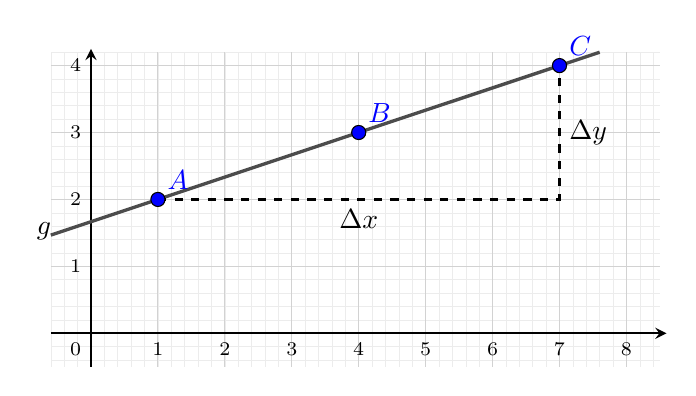
\begin{tikzpicture}[scale=0.85,>=stealth]
                  % Raster
                  \draw[step=0.2,gray!15,very thin]
                  (-0.6,-0.5) grid (8.5,4.2);
                  \draw[step=1,gray!35,thin]
                  (-0.6,-0.5) grid (8.5,4.2);

                  % Achsen
                  \draw[->,thick] (-0.6,0) -- (8.6,0);
                  \draw[->,thick] (0,-0.5) -- (0,4.25);

                  \foreach \x in {1,...,8}
                  \node[below,font=\scriptsize] at (\x,0) {\(\x\)};
                  \foreach \y in {1,...,4}
                  \node[left,font=\scriptsize] at (0,\y) {\(\y\)};
                  \node[below left,font=\scriptsize] at (0,0) {\(0\)};

                  % Gerade
                  \draw[black!70,very thick]
                  (-0.6,1.4667) -- (7.6,4.2);
                  \node[left] at (-0.45,1.52) {\(g\)};

                  % Steigungsdreieck
                  \draw[thick,dashed]
                  (1,2) -- (7,2) -- (7,4);

                  % Punkte
                  \foreach \x/\y/\name in {1/2/A,4/3/B,7/4/C} {
                          \filldraw[blue,draw=black]
                          (\x,\y) circle (3pt);
                          \node[blue,above right] at (\x,\y) {\(\name\)};
                      }

                  \node[below] at (4,2) {\(\Delta x\)};
                  \node[right] at (7,3) {\(\Delta y\)};
              \end{tikzpicture}
          \end{center}

          \[
              \frac{\Delta y}{\Delta x}
              = \frac{4-2}{7-1}
              = \frac26
              = \frac13.
          \]

          Weil die beiden verwendeten Dreiecke -- die sogenannten
          \emph{Steigungsdreiecke} -- ähnlich sind, ist das Verhältnis
          der beiden Katheten in beiden gleich.


    \item Eine Gerade ist genau dann streng monoton wachsend
          (bzw. fallend), wenn ihre Steigung positiv (bzw. negativ) ist.


          Die Gerade im folgenden Bild hat die Steigung

          \[
              \frac{\Delta y}{\Delta x}
              = \frac{y_B-y_A}{x_B-x_A}
              = \frac{-2-2}{7-1}
              = \frac{-4}{6}
              = -\frac23.
          \]

          \begin{center}
              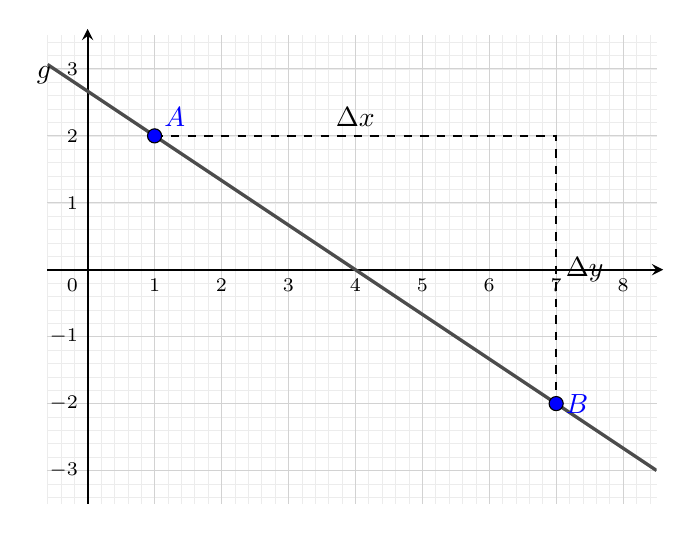
\begin{tikzpicture}[scale=0.85,>=stealth]
                  % Raster
                  \draw[step=0.2,gray!15,very thin]
                  (-0.6,-3.5) grid (8.5,3.5);
                  \draw[step=1,gray!35,thin]
                  (-0.6,-3.5) grid (8.5,3.5);

                  % Achsen
                  \draw[->,thick] (-0.6,0) -- (8.6,0);
                  \draw[->,thick] (0,-3.5) -- (0,3.6);

                  \foreach \x in {1,...,8}
                  \node[below,font=\scriptsize] at (\x,0) {\(\x\)};
                  \foreach \y in {-3,-2,-1,1,2,3}
                  \node[left,font=\scriptsize] at (0,\y) {\(\y\)};
                  \node[below left,font=\scriptsize] at (0,0) {\(0\)};

                  % Gerade
                  \begin{scope}
                      \clip (-0.6,-3.5) rectangle (8.5,3.5);
                      \draw[black!70,very thick]
                      (-0.6,3.0667) -- (8.5,-3);
                  \end{scope}
                  \node[left] at (-0.4,2.9) {\(g\)};

                  % Steigungsdreieck
                  \draw[thick,dashed]
                  (1,2) -- (7,2) -- (7,-2);

                  % Punkte
                  \filldraw[blue,draw=black] (1,2) circle (3pt);
                  \filldraw[blue,draw=black] (7,-2) circle (3pt);

                  \node[blue,above right] at (1,2) {\(A\)};
                  \node[blue,right] at (7,-2) {\(B\)};

                  \node[above] at (4,2) {\(\Delta x\)};
                  \node[right] at (7,0) {\(\Delta y\)};
              \end{tikzpicture}
          \end{center}

    \item Eine Gerade mit der Steigung \(1=100\,\%\) ist um
          \(45^\circ\) gegenüber der Horizontalen geneigt.
\end{itemize}

\begin{center}
    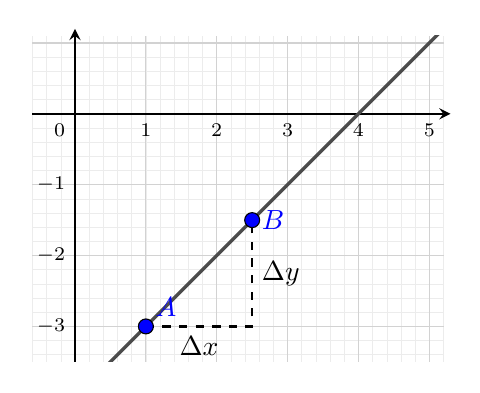
\begin{tikzpicture}[scale=0.9,>=stealth]
        % Raster
        \draw[step=0.2,gray!15,very thin]
        (-0.6,-3.5) grid (5.2,1.1);
        \draw[step=1,gray!35,thin]
        (-0.6,-3.5) grid (5.2,1.1);

        % Achsen
        \draw[->,thick] (-0.6,0) -- (5.3,0);
        \draw[->,thick] (0,-3.5) -- (0,1.2);

        \foreach \x in {1,...,5}
        \node[below,font=\scriptsize] at (\x,0) {\(\x\)};
        \foreach \y in {-3,-2,-1}
        \node[left,font=\scriptsize] at (0,\y) {\(\y\)};
        \node[below left,font=\scriptsize] at (0,0) {\(0\)};

        % Gerade y = x - 4
        \begin{scope}
            \clip (-0.6,-3.5) rectangle (5.2,1.1);
            \draw[black!70,very thick]
            (0,-4) -- (5.2,1.2);
        \end{scope}

        % Steigungsdreieck
        \draw[thick,dashed]
        (1,-3) -- (2.5,-3) -- (2.5,-1.5);

        % Punkte
        \filldraw[blue,draw=black] (1,-3) circle (3pt);
        \filldraw[blue,draw=black] (2.5,-1.5) circle (3pt);

        \node[blue,above right] at (1,-3) {\(A\)};
        \node[blue,right] at (2.5,-1.5) {\(B\)};

        \node[below] at (1.75,-3) {\(\Delta x\)};
        \node[right] at (2.5,-2.25) {\(\Delta y\)};
    \end{tikzpicture}
\end{center}

\[
    \frac{\Delta y}{\Delta x}
    = \frac{y_B-y_A}{x_B-x_A}
    = \frac{-1.5-(-3)}{2.5-1}
    = \frac{1.5}{1.5}
    = 1
    = 100\,\%.
\]

\begin{itemize}
    \item Für vertikale Geraden gilt \(\Delta x=0\).
          Aus diesem Grund hat eine vertikale Gerade keine Steigung.

    \item \textbf{Merkspruch:}

          \centering\emph{Steigung = \enquote{Obsi pro Vorwärts}}
\end{itemize}






\clearpage
\subsection{Der Graph einer linearen Funktion}
\begin{LA}
    {Einführungsaufgabe}{}
    \begin{enumerate}
        \item Liegen die Punkte \(A=(1|2)\), \(B=(8|4)\) und
              \(C=(18|7)\) auf einer Geraden?
              Tipp: Betrachten Sie die Steigung.

        \item Gegeben ist die Funktion \(f(x)=2x+6\).

              \begin{enumerate}
                  \item Bestimmen Sie die Koordinaten von drei Punkten
                        auf dem Graphen von \(f\). Zeigen Sie, dass sie
                        auf einer Geraden liegen.

                  \item Wieso reicht die Aufgabe a) nicht als Beweis
                        dafür, dass der Graph von \(f\) eine Gerade ist?

                  \item \textbf{Challenge:}
                        Betrachten Sie nun zwei allgemeine Punkte
                        \(A=(x_A|y_A)\) und \(B=(x_B|y_B)\)
                        auf dem Graphen von \(f\).

                        \begin{enumerate}
                            \item[i)] Erklären Sie, wieso
                                  \(y_A=2x_A+6\) sein muss.

                            \item[ii)] Berechnen Sie die Steigung und formen
                                  Sie den Term so lange um, bis Sie eine Zahl erhalten.
                        \end{enumerate}
              \end{enumerate}
    \end{enumerate}
\end{LA}

\clearpage
\begin{satz}{Der Graph ist eine Gerade!}{}
    Der Graph einer linearen Funktion der Form
    \(f(x)=ax+b\) ist eine Gerade mit dem
    \(y\)-Achsenabschnitt \(b\) und der Steigung \(a\).

    \begin{center}
        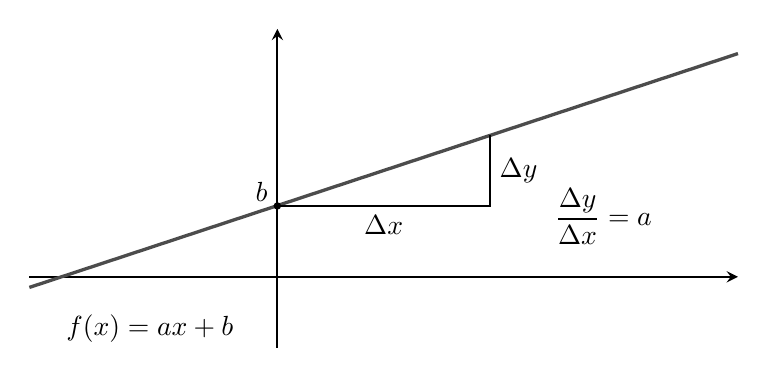
\begin{tikzpicture}[scale=0.9,>=stealth]

            % Achsen
            \draw[->,thick] (-3.5,0) -- (6.5,0);
            \draw[->,thick] (0,-1) -- (0,3.5);

            % Gerade f(x) = ax+b (schematisch)
            \draw[black!70,very thick]
            (-3.5,-0.15) -- (6.5,3.15);

            % y-Achsenabschnitt
            \fill (0,1) circle (1.5pt);
            \node[left] at (0,1.2) {\(b\)};

            % Steigungsdreieck
            \draw[thick]
            (0,1) -- (3,1) -- (3,2);

            % Beschriftungen
            \node[below] at (1.5,1) {\(\Delta x\)};
            \node[right] at (3,1.5) {\(\Delta y\)};

            \node at (4.6,0.85)
            {\(\displaystyle\frac{\Delta y}{\Delta x}=a\)};

            \node[below] at (-1.8,-0.4) {\(f(x)=ax+b\)};

        \end{tikzpicture}
    \end{center}
\end{satz}


\medskip
\begin{proof}

    Zuerst wird bewiesen, dass der \(y\)-Achsenabschnitt \(b\) ist.
    Zur Erinnerung: Der \(y\)-Achsenabschnitt ist der Funktionswert
    an der Stelle 0. In diesem Fall also:
    \[
        f(0)=a\cdot 0+b=b.
    \]

    Nun wird gezeigt, dass der Graph von \(f\) eine Gerade ist:
    Seien \(A=(x_A|y_A)\) und \(B=(x_B|y_B)\) zwei
    \emph{beliebige} Punkte auf dem Graphen von \(f\)
    mit \(x_A\neq x_B\).
    Das heisst: \(y_A=f(x_A)\) und \(y_B=f(x_B)\).
    Die Steigung der Verbindungsstrecke zwischen \(A\) und \(B\)
    beträgt dann:

    \begin{align*}
        \frac{\Delta y}{\Delta x}
         & = \frac{y_B-y_A}{x_B-x_A}               \\
         & = \frac{f(x_B)-f(x_A)}{x_B-x_A}         \\
         & = \frac{(a\cdot x_B+b)-(a\cdot x_A+b)}
             {x_B-x_A}   \\
         & = \frac{a\cdot x_B-a\cdot x_A}{x_B-x_A} \\
         & = \frac{a\cdot(x_B-x_A)}{x_B-x_A}       \\
         & = a.
    \end{align*}

    Die Steigung zwischen zwei Graphenpunkten ist demnach
    immer dieselbe, nämlich \(a\).
    Damit muss der Graph eine Gerade mit der Steigung \(a\) sein.
\end{proof}












\clearpage
\subsection{Funktionsgleichung \(\longleftrightarrow\) Graph}

\begin{bsp}
    {Gleichung \(\longrightarrow\) Graph}{}
    \textbf{Gegeben} ist die Funktionsgleichung
    \(
    f(x) = -\frac{2}{3}x + 1.
    \)

    \textbf{Gesucht} ist der Graph der Funktion.

    \karofeld{7.2cm}
\end{bsp}

\begin{bsp}
    {Gleichung \(\longleftarrow\) Graph}{}
    \textbf{Gegeben} sind \(P=(0|1)\) und \(Q=(2|4)\)
    auf dem Graphen der linearen Funktion \(g\).

    \textbf{Gesucht} ist die Funktionsgleichung.

    \karofeld{9.2cm}
\end{bsp}

\begin{bsp}
    {Anwendung}{}
    Bei einer Prüfung erhält man für 0 Punkte die Note 1.
    Für 17 Punkte die Note 6. Dazwischen ist die Notenskala linear.

    Wie lautet die Gleichung der Funktion
    \[
        N\colon [0,17] \to [1,6],
    \]
    die jeder Punktzahl \(p\) die entsprechende Note \(N(p)\) zuordnet?

    \karofeld{16}
\end{bsp}


\begin{bsp}
    {Anwendung}{}
    Für welche lineare Funktion \(f\) gilt \(f(1) = 2\) und \(f(6) = 5\)?

    \karofeld{18}
\end{bsp}


\clearpage
\begin{ueb}
    {Gleichung und Graph}{}
    \begin{enumerate}

        \item Zeichnen Sie die Geraden mit den angegebenen Funktionsgleichungen
              nur anhand des \(y\)-Achsenabschnitts \(b\) und der Steigung \(a\)
              in ein Koordinatensystem.

              \begin{enumerate}
                  \item \(y=2x+3\)
                  \item \(y=-3x-1\)
                  \item \(y=\frac{3}{5}x+\frac{5}{2}\)
                  \item \(y=-\frac{5}{3}x-\frac{2}{5}\)
              \end{enumerate}
        \item Geben Sie für jede eingezeichnete Gerade die Funktionsgleichung an.

              \begin{enumerate}
                  \item
                        \begin{center}
                            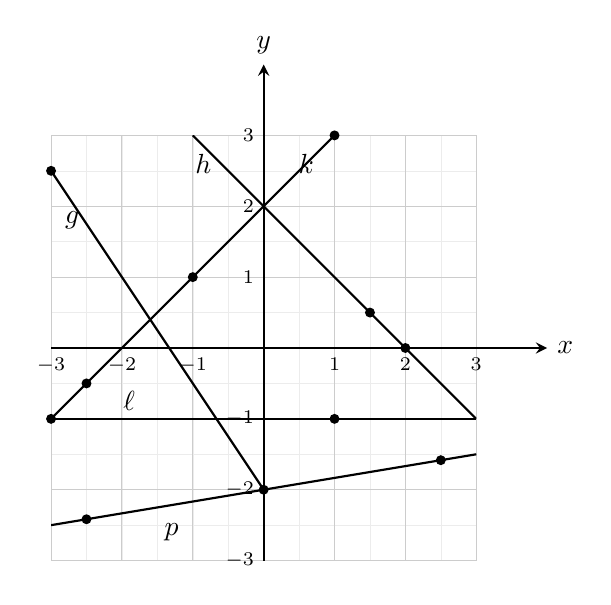
\begin{tikzpicture}[scale=0.9,>=stealth]
                                % Raster
                                \draw[step=0.5,gray!15,very thin]
                                (-3,-3) grid (3,3);
                                \draw[step=1,gray!40,thin]
                                (-3,-3) grid (3,3);

                                % Achsen
                                \draw[->,thick] (-3,0) -- (4,0)
                                node[right] {\(x\)};
                                \draw[->,thick] (0,-3) -- (0,4)
                                node[above] {\(y\)};

                                % Achsenbeschriftungen
                                \foreach \x in {-3,-2,-1,1,2,3}
                                \node[below,font=\scriptsize] at (\x,0) {\(\x\)};
                                \foreach \y in {-3,-2,-1,1,2,3}
                                \node[left,font=\scriptsize] at (0,\y) {\(\y\)};

                                % Geraden
                                \begin{scope}
                                    \clip (-3,-3) rectangle (3,3);

                                    % g
                                    \draw[thick] (-3,2.5) -- (0,-2);

                                    % h
                                    \draw[thick] (-1,3) -- (3,-1);

                                    % k
                                    \draw[thick] (-3,-1) -- (1,3);

                                    % l
                                    \draw[thick] (-3,-1) -- (3,-1);

                                    % p
                                    \draw[thick] (-3,-2.5) -- (3,-1.5);
                                \end{scope}

                                % Markierte Punkte
                                \foreach \x/\y in {
                                        -3/2.5,0/-2,
                                        1.5/0.5,2/0,
                                        -3/-1,-2.5/-0.5,-1/1,1/3,
                                        1/-1,
                                        -2.5/-2.4167,2.5/-1.5833
                                    } {
                                        \fill (\x,\y) circle (2pt);
                                    }

                                % Beschriftungen
                                \node at (-2.7,1.8) {\(g\)};
                                \node at (-0.85,2.6) {\(h\)};
                                \node at (0.6,2.6) {\(k\)};
                                \node at (-1.9,-0.75) {\(\ell\)};
                                \node at (-1.3,-2.6) {\(p\)};

                            \end{tikzpicture}
                        \end{center}

                  \item
                        \begin{center}
                            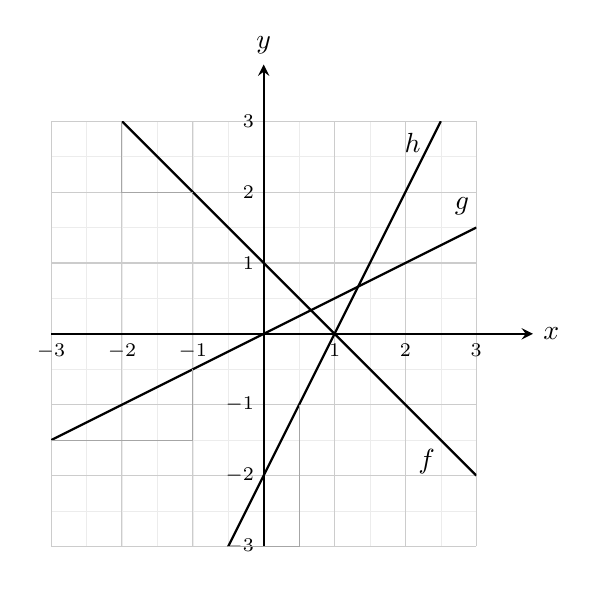
\begin{tikzpicture}[scale=0.9,>=stealth]
                                % Raster
                                \draw[step=0.5,gray!15,very thin]
                                (-3,-3) grid (3,3);
                                \draw[step=1,gray!40,thin]
                                (-3,-3) grid (3,3);

                                % Achsen
                                \draw[->,thick] (-3,0) -- (3.8,0)
                                node[right] {\(x\)};
                                \draw[->,thick] (0,-3) -- (0,3.8)
                                node[above] {\(y\)};

                                % Achsenbeschriftungen
                                \foreach \x in {-3,-2,-1,1,2,3}
                                \node[below,font=\scriptsize] at (\x,0) {\(\x\)};
                                \foreach \y in {-3,-2,-1,1,2,3}
                                \node[left,font=\scriptsize] at (0,\y) {\(\y\)};

                                % Geraden
                                \begin{scope}
                                    \clip (-3,-3) rectangle (3,3);

                                    % f
                                    \draw[thick] (-2,3) -- (3,-2);

                                    % g
                                    \draw[thick] (-3,-1.5) -- (3,1.5);

                                    % h
                                    \draw[thick] (-0.5,-3) -- (2.5,3);
                                \end{scope}

                                % Steigungsdreiecke
                                \draw[gray!70,thin]
                                (-2,3) -- (-2,2) -- (-1,2);

                                \draw[gray!70,thin]
                                (-3,-1.5) -- (-1,-1.5) -- (-1,-0.5);

                                \draw[gray!70,thin]
                                (-0.5,-3) -- (0.5,-3) -- (0.5,-1);

                                % Beschriftungen
                                \node at (2.3,-1.8) {\(f\)};
                                \node at (2.8,1.8) {\(g\)};
                                \node at (2.1,2.7) {\(h\)};

                            \end{tikzpicture}
                        \end{center}
              \end{enumerate}
        \item Die Punkte \(A\) und \(B\) liegen auf einer Geraden.
              Geben Sie deren Funktionsgleichung an.
              \begin{enumerate}
                  \item \(A=(0|0),\quad B=(1|-2)\)
                  \item \(A=(-7|3),\quad B=(11|3)\)
                  \item \(A=(-2|5),\quad B=(3|20)\)
              \end{enumerate}

        \item Von der Funktion \(f(x)=ax+b\) mit \(a=\frac{2}{3}\)
              ist \(f(-6)=0\) bekannt.
              Berechnen Sie \(b\) und \(f(10)\).

        \item Von der Funktion \(f(x)=ax+4\) ist \(f(5)=9\) bekannt.
              Berechnen Sie \(a\) und \(f(-5)\).

        \item Eine lineare Funktion hat die Gleichung
              \(f(x)=\frac{1}{3}x-2\).
              Bestimmen Sie \(f(0)\), \(f(-4)\) und \(f(27)\).

              Für welche Stelle \(x\) gilt \(f(x)=3\) bzw. \(f(x)=-5\)?
        \item Gegeben sind die Funktionen
              \(f_1(x)=-\frac{1}{2}x\),
              \(f_2(x)=-2x+2\) und
              \(f_3(x)=\frac{5}{2}x-\frac{2}{3}\).

              \begin{enumerate}
                  \item Welche Funktion hat als Graph eine Gerade durch
                        den Ursprung \((0|0)\)?

                  \item Welche Funktion hat als Graph eine Gerade mit
                        einer Steigung grösser als 2?

                  \item Welche Funktion hat als Graph eine Gerade
                        parallel zur \(x\)-Achse?

                  \item Schneiden die Graphen der Funktionen \(f_1\)
                        und \(f_3\) einander?
              \end{enumerate}
        \item \textbf{Challenge:} Gegeben sind die Geraden \(g: y=3x\) und
              \(h: y=-\frac{1}{2}x-1\).

              \begin{enumerate}
                  \item Die Graphen von \(g\) und \(h\) werden an der
                        \(y\)-Achse gespiegelt.
                        Geben Sie die Funktionsgleichungen der Bildgeraden an.

                  \item Die Graphen von \(g\) und \(h\) werden an der
                        \(x\)-Achse gespiegelt.
                        Geben Sie die Funktionsgleichungen der Bildgeraden an.

                  \item Die Graphen von \(g\) und \(h\) werden am
                        Koordinatenursprung gespiegelt.
                        Geben Sie die Funktionsgleichungen der Bildgeraden an.
              \end{enumerate}
    \end{enumerate}
\end{ueb}

\clearpage
\textbf{Lösungen:}
\begin{enumerate}
    \item
          \begin{enumerate}
              \item \(a=2,\quad b=3\)
              \item \(a=-3,\quad b=-1\)
              \item \(a=\frac35,\quad b=\frac52\)
              \item \(a=-\frac53,\quad b=-\frac25\)
          \end{enumerate}

    \item
          \begin{enumerate}
              \item
                    \[
                        \begin{aligned}
                            g(x)    & =-\frac32x-2 \\
                            h(x)    & =-x+2        \\
                            k(x)    & =x+2         \\
                            \ell(x) & =-1          \\
                            p(x)    & =\frac16x-2
                        \end{aligned}
                    \]

              \item
                    \[
                        \begin{aligned}
                            f(x) & =-x+1     \\
                            g(x) & =\frac12x \\
                            h(x) & =2x-2
                        \end{aligned}
                    \]
          \end{enumerate}

    \item
          \begin{enumerate}

              \item \(y=-2x\)
              \item \(y=3\)
              \item \(y=3x+11\).
          \end{enumerate}

    \item
          \[
              0=\frac23\cdot(-6)+b
              \quad\Rightarrow\quad b=4
          \]
          \[
              f(10)=\frac23\cdot10+4=\frac{32}{3}
          \]

    \item
          \[
              9=5a+4
              \quad\Rightarrow\quad a=1
          \]
          \[
              f(-5)=-5+4=-1
          \]

    \item
          \[
              f(0)=-2,\qquad
              f(-4)=-\frac{10}{3},\qquad
              f(27)=7
          \]
          \[
              f(x)=3\ \Rightarrow\ x=15,
              \qquad
              f(x)=-5\ \Rightarrow\ x=-9
          \]

    \item
          \begin{enumerate}
              \item \(f_1\)
              \item \(f_3\), da \(a=\frac52>2\).
              \item Keine der drei Funktionen.
              \item Ja, da die Steigungen verschieden sind.
                    % Der Schnittpunkt ist
                    % \[
                    %     S=\left(\frac29\middle|-\frac19\right).
                    % \]
          \end{enumerate}

    \item \textbf{Challenge:}
          \begin{enumerate}
              \item Spiegelung an der \(y\)-Achse:
                    \[
                        g'(x)=-3x,\qquad
                        h'(x)=\frac12x-1
                    \]

              \item Spiegelung an der \(x\)-Achse:
                    \[
                        g'(x)=-3x,\qquad
                        h'(x)=\frac12x+1
                    \]

              \item Spiegelung am Ursprung:
                    \[
                        g'(x)=3x,\qquad
                        h'(x)=-\frac12x+1
                    \]
          \end{enumerate}
\end{enumerate}









\clearpage
\subsection{Anwendungen}

Ganz am Anfang des Themas Funktionen wurde erwähnt, dass es sich
dabei um \enquote{mentale Werkzeuge} handelt. Damit ist gemeint,
dass man viele Fragestellungen mit einer \enquote{Funktionenbrille}
betrachten kann und dann Analogien zwischen Problemen entstehen,
die auf den ersten Blick nicht viel gemeinsam haben.

Eine wesentliche Grundlage des Erfolgs von Newton in der Mechanik
beruht darauf, dass er Bewegung als eine Funktion betrachtet hat.

\begin{LA}
    {Weg-Zeit-Diagramm}{}

    Eine Person bewegt sich entlang einer geraden Strecke.
    \begin{center}
        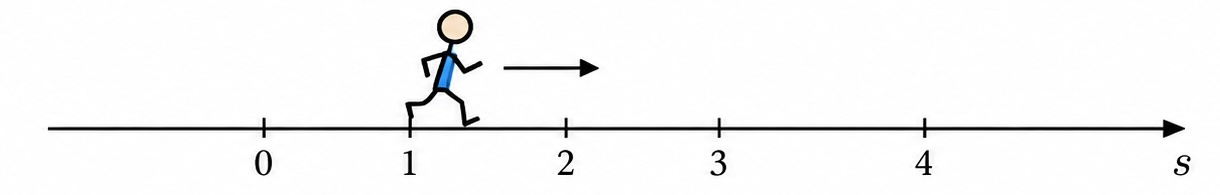
\includegraphics[width=0.5\textwidth]{media/rennen_entlang_achse.jpg}
    \end{center}
    Dabei wird jedem Zeitpunkt \(t\) eine Position \(s\) zugeordnet.

    \[
        \text{Zeit } t \longmapsto \text{Position } s
    \]

    \begin{center}
        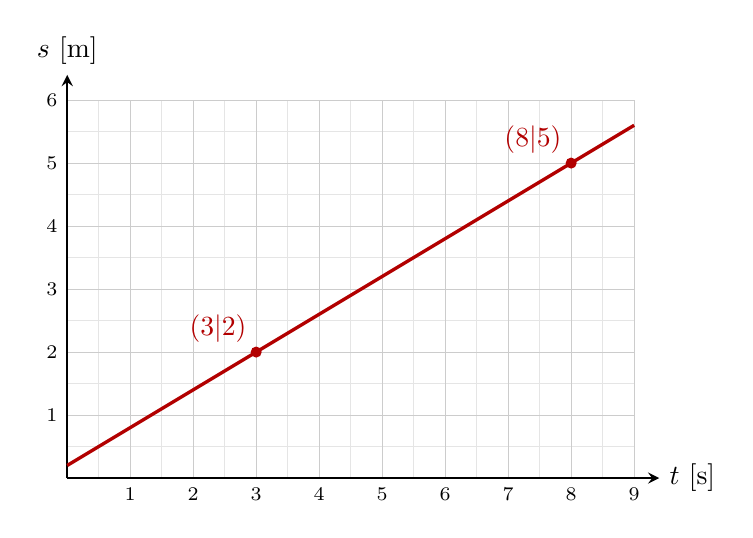
\begin{tikzpicture}[scale=0.8, >=stealth]

            % Feines Raster
            \draw[step=0.5, gray!20, very thin]
            (0,0) grid (9,6);

            % Hauptgitter
            \draw[step=1, gray!40, thin]
            (0,0) grid (9,6);

            % Achsen
            \draw[->, thick] (0,0) -- (9.4,0)
            node[right] {\(t\) [s]};

            \draw[->, thick] (0,0) -- (0,6.4)
            node[above] {\(s\) [m]};

            % Achsenbeschriftungen
            \foreach \x in {1,...,9} {
                    \node[below, font=\scriptsize] at (\x,0) {\(\x\)};
                }

            \foreach \y in {1,...,6} {
                    \node[left, font=\scriptsize] at (0,\y) {\(\y\)};
                }

            % Gerade durch (3,2) und (8,5)
            % Steigung = 3/5, Achsenabschnitt = 1/5
            \draw[red!70!black, very thick]
            (0,0.2) -- (9,5.6);

            % Punkte
            \fill[red!70!black] (3,2) circle (2.5pt);
            \fill[red!70!black] (8,5) circle (2.5pt);

            % Punktbeschriftungen
            \node[red!70!black, above left] at (3,2)
            {\((3|2)\)};

            \node[red!70!black, above left] at (8,5)
            {\((8|5)\)};

        \end{tikzpicture}
    \end{center}

    \begin{enumerate}
        \item Welche Bedeutung haben die Graphenpunkte
              \((3|2)\) und \((8|5)\)?

        \item Bestimmen Sie die Geschwindigkeit der Person.
    \end{enumerate}
\end{LA}

\clearpage
\begin{ueb}{Alice und Bob auf dem Weg zum Flughafen}{}

    Alice fährt mit dem Elektrovelo mit einer konstanten Geschwindigkeit
    von \(v_A=\SI{20}{\kilo\meter\per\hour}\) in Richtung Flughafen.

    Zum Zeitpunkt \(t=0\) fährt sie am Ortsausgangsschild bei
    Winterthur-Töss vorbei.

    Bob will Alice mit dem Roller einholen. Er fährt mit konstanter
    Geschwindigkeit \(v_B=\SI{80}{\kilo\meter\per\hour}\) und passiert
    das Ortsausgangsschild 30 Minuten nach Alice.

    \begin{enumerate}
        \item Geben Sie die Gleichungen der Funktionen \(s_A(t)\)
              und \(s_B(t)\) an, welche jedem Zeitpunkt \(t\)
              (in Minuten) die Entfernung (in Kilometern) von Alice
              bzw. Bob vom Ortsausgangsschild zuordnen.

              \emph{Tipp:} Bestimmen Sie zuerst die beiden
              Geschwindigkeiten in \(\si{\kilo\meter\per\minute}\).

              %   \vspace{3cm}

        \item Zeichnen Sie die beiden Graphen in das Koordinatensystem.

              \begin{center}
                  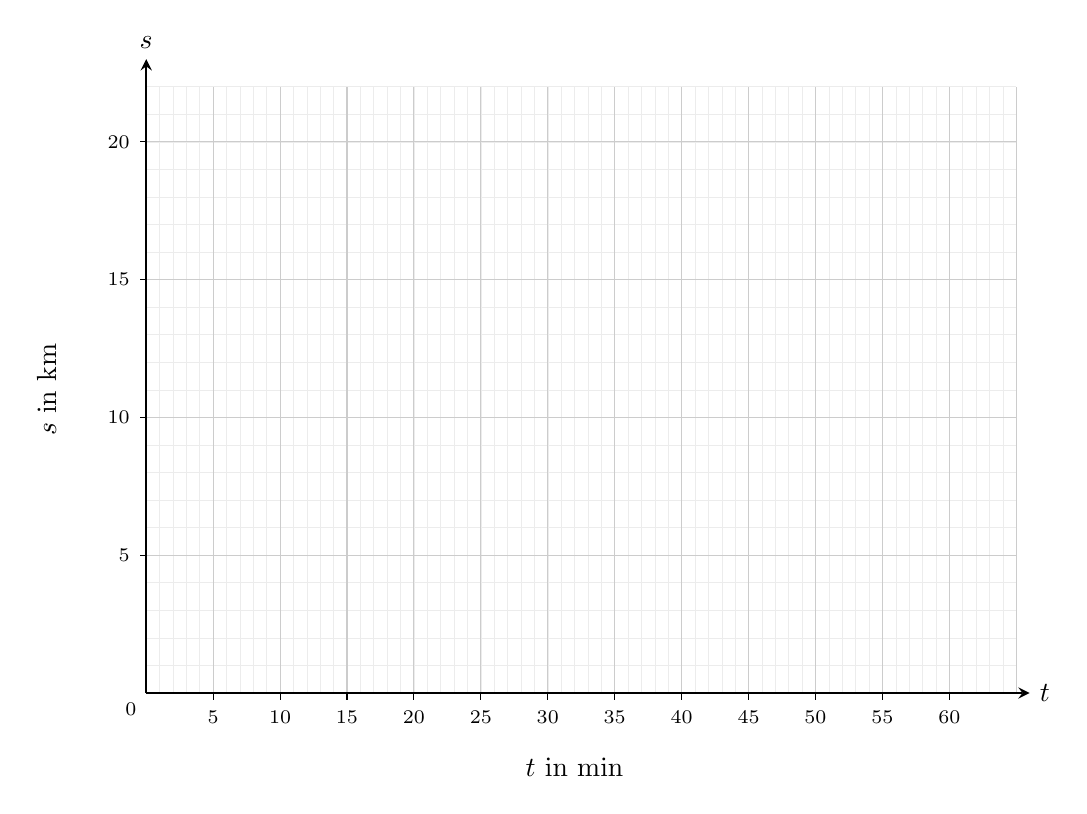
\begin{tikzpicture}[
                          x=0.17cm,
                          y=0.35cm,
                          >=stealth
                      ]

                      % Feines Raster: 1 min / 1 km
                      \draw[step=1, gray!15, very thin]
                      (0,0) grid (65,22);

                      % Hauptgitter: 5 min / 5 km
                      \foreach \x in {0,5,...,65} {
                              \draw[gray!40, thin]
                              (\x,0) -- (\x,22);
                          }

                      \foreach \y in {0,5,...,20} {
                              \draw[gray!40, thin]
                              (0,\y) -- (65,\y);
                          }

                      % Achsen
                      \draw[->, thick]
                      (0,0) -- (66,0)
                      node[right] {\(t\)};

                      \draw[->, thick]
                      (0,0) -- (0,23)
                      node[above] {\(s\)};

                      % Horizontale Achse
                      \foreach \x in {5,10,...,60} {
                              \draw (\x,0) -- (\x,-0.25);
                              \node[below, font=\scriptsize]
                              at (\x,-0.3) {\x};
                          }

                      % Vertikale Achse
                      \foreach \y in {5,10,15,20} {
                              \draw (0,\y) -- (-0.5,\y);
                              \node[left, font=\scriptsize]
                              at (-0.5,\y) {\y};
                          }

                      % Ursprung
                      \node[below left, font=\scriptsize]
                      at (0,0) {0};

                      % Einheiten
                      \node[below] at (32,-2) {\(t\) in min};
                      \node[rotate=90, above] at (-6,11)
                      {\(s\) in km};

                  \end{tikzpicture}
              \end{center}

        \item Zu welchem Zeitpunkt und in welcher Entfernung von
              Töss wird Alice von Bob eingeholt?

              Schafft es Bob, Alice einzuholen, bevor sie am
              \(\SI{13.5}{\kilo\meter}\) entfernten Flughafen eintrifft?

    \end{enumerate}


\end{ueb}

\clearpage
\begin{ueb}{Anwendungsaufgaben zu linearen Funktionen}{}
    \begin{enumerate}
        \item Ein Elektro-Fachgeschäft verkauft verschieden lange Kabel
              auf identischen Kabelrollen. Eine 20-m-Rolle wiegt
              \qty{4.2}{\kilo\gram} und eine 50-m-Rolle wiegt
              \qty{9.3}{\kilo\gram}.

              Bestimmen Sie die lineare Funktion \(f\), die der
              Kabellänge \(\ell\) das Gesamtgewicht \(G\) der Rolle
              zuordnet.

        \item In einer Deutschprüfung mit total 34 Punkten ergeben
              0 Punkte die Note 1 und 32.5 Punkte die Note 6.
              Es gibt nur ganze und halbe Punkte und Noten.
              Die Notenskala ist linear.

              \begin{enumerate}
                  \item Geben Sie die Gleichung der Funktion an,
                        die jeder Punktzahl \(P\) die Note \(N\)
                        zuordnet.

                  \item Welche Note erhält Mia für 25 Punkte?

                  \item Welche Punktzahl benötigt Leon mindestens,
                        um die Note 4 zu erhalten?
              \end{enumerate}

        \item Jan fährt um 8.00 Uhr mit seinem Fahrrad Richtung
              St. Gallen los und fährt mit einer konstanten
              Geschwindigkeit von \qty{12}{\kilo\meter\per\hour}.

              Seine Schwester Emma fährt ihm ab 10.30 Uhr mit
              ihrem Roller mit \qty{30}{\kilo\meter\per\hour} nach.

              Wann muss Maria den beiden vom
              \qty{60}{\kilo\meter} entfernten St. Gallen zu Fuss
              mit \qty{5}{\kilo\meter\per\hour} entgegenlaufen,
              wenn sie zur gleichen Zeit wie Jan und Emma an
              deren Treffpunkt sein will?

              Lösen Sie die Aufgabe grafisch und überprüfen Sie
              Ihr Ergebnis rechnerisch.
    \end{enumerate}
\end{ueb}

\clearpage
\textbf{Kurzlösungen}

\begin{enumerate}
    \item
          \[
              {G(l)=0.17\cdot l+0.8}
          \]

    \item Notenskala:
          \begin{enumerate}
              \item
                    \[
                        {N(P)=1+\frac{2}{13}P}
                    \]

              \item
                    \[
                        N(25)=\frac{63}{13}\approx4.85
                    \]


              \item
                    \[
                        1+\frac{2}{13}P=4
                        \quad\Longrightarrow\quad P=19.5
                    \]

          \end{enumerate}

    \item

          Sie muss um \({10.10\text{ Uhr}}\) loslaufen.
\end{enumerate}




































\clearpage
\subsection{Einblick in die analytische Geometrie}
\begin{LA}
    {}{Quadrat?}
    Zeichnen Sie die Graphen der vier gegebenen Funktionen
    in das Koordinatensystem ein.

    \[
        \begin{aligned}
            f_1(x) & = 2x+3,               &
            f_2(x) & = -\frac12 x+\frac32,   \\[4pt]
            f_3(x) & = 2x-3,               &
            f_4(x) & = -\frac12 x-\frac32.
        \end{aligned}
    \]

    \begin{center}
        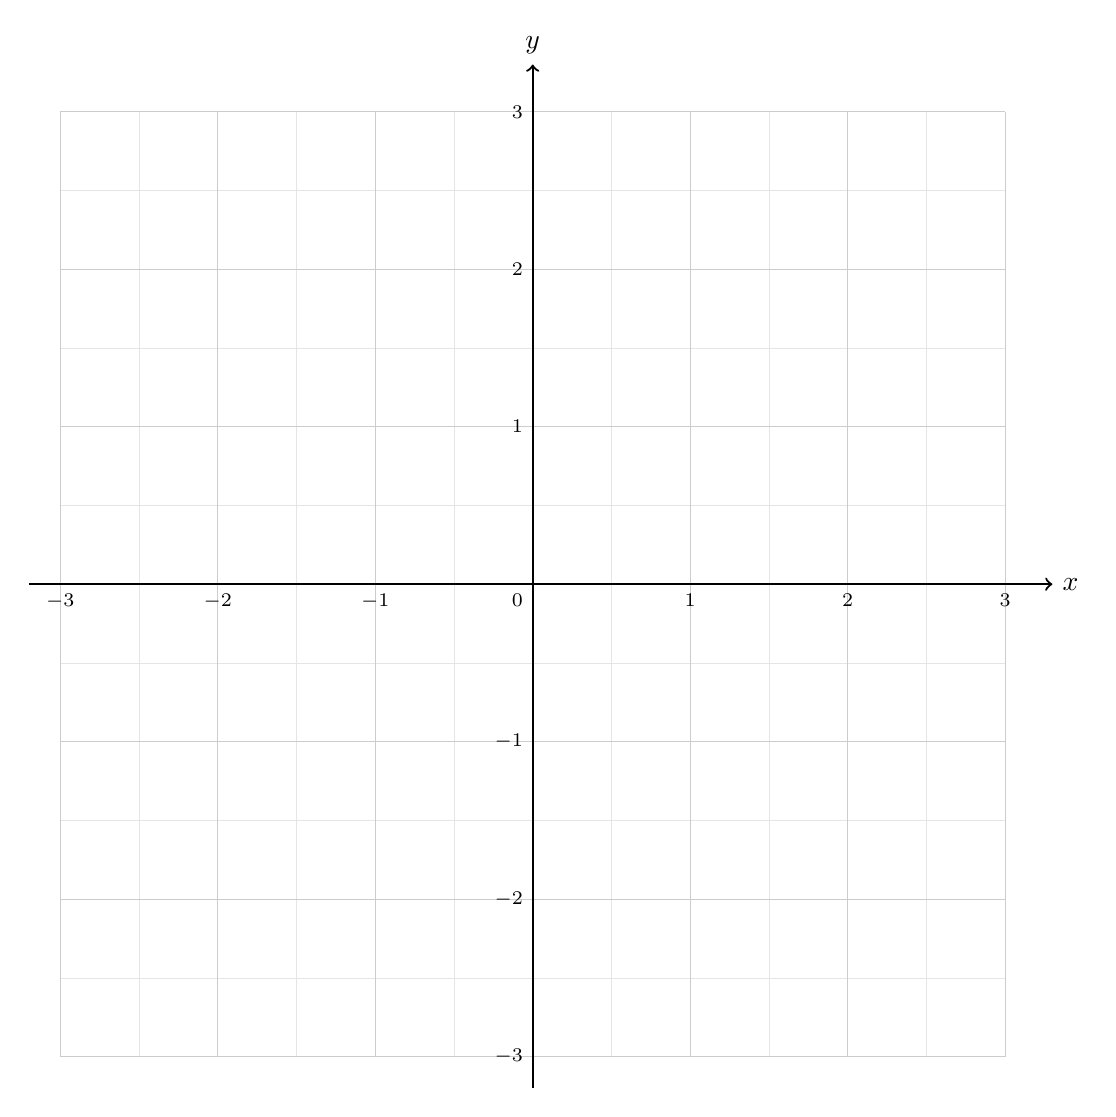
\begin{tikzpicture}[scale=2]
            % Feines Gitter (0.5 Einheiten)
            \draw[step=0.5,gray!20,very thin]
            (-3,-3) grid (3,3);

            % Hauptgitter (1 Einheit)
            \draw[step=1,gray!40,thin]
            (-3,-3) grid (3,3);

            % Koordinatenachsen
            \draw[->,thick] (-3.2,0) -- (3.3,0)
            node[right] {\(x\)};
            \draw[->,thick] (0,-3.2) -- (0,3.3)
            node[above] {\(y\)};

            % Achsenbeschriftungen
            \foreach \x in {-3,-2,-1,1,2,3} {
                    \node[below,font=\scriptsize]
                    at (\x,0) {\(\x\)};
                }

            \foreach \y in {-3,-2,-1,1,2,3} {
                    \node[left,font=\scriptsize]
                    at (0,\y) {\(\y\)};
                }

            % Ursprung
            \node[below left,font=\scriptsize]
            at (0,0) {\(0\)};

        \end{tikzpicture}
    \end{center}

    Was vermuten Sie? Was davon können Sie schon begründen? Was müsste man noch prüfen?
\end{LA}

\clearpage


René Descartes (1596--1650) gilt als Begründer der
\emph{analytischen Geometrie}, dem Bindeglied zwischen
Geometrie und Algebra.

\begin{center}
    \includegraphics[width = 0.25\textwidth]{media/Frans_Hals_-_Portret_van_René_Descartes.jpg}
\end{center}

In seinem Werk \enquote{Discours de la méthode pour bien conduire
    sa raison et chercher la vérité dans les sciences} verwendet er
systematisch Koordinatensysteme, um geometrische Probleme in die
Algebra einzubetten. Punkte werden durch ihre Koordinaten und
Geraden, Kreise oder andere Kurven durch Gleichungen beschrieben.
Dadurch lassen sich geometrische Fragen neu mit den Werkzeugen
der Arithmetik bearbeiten!

\medskip

\textbf{Punkte:} Jeder Punkt im Koordinatensystem entspricht
einem Zahlenpaar \((x|y)\) und umgekehrt.

Beispiel: Der Punkt \(A\) in der Skizze entspricht dem
Zahlenpaar \((-2|1)\).

\begin{center}
    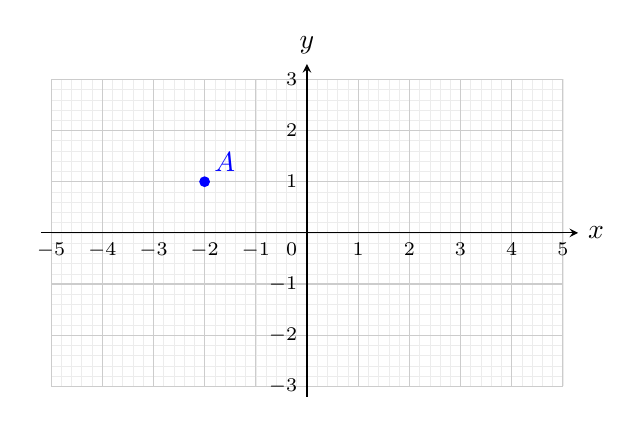
\begin{tikzpicture}[scale=0.65,>=stealth]
        % Raster
        \draw[step=0.2,gray!15,very thin]
        (-5,-3) grid (5,3);
        \draw[step=1,gray!40,thin]
        (-5,-3) grid (5,3);

        % Achsen
        \draw[->] (-5.2,0) -- (5.3,0) node[right] {\(x\)};
        \draw[->] (0,-3.2) -- (0,3.3) node[above] {\(y\)};

        % Beschriftungen
        \foreach \x in {-5,...,5} {
                \ifnum\x=0\relax\else
                    \node[below,font=\scriptsize] at (\x,0) {\(\x\)};
                \fi
            }
        \foreach \y in {-3,-2,-1,1,2,3} {
                \ifnum\y=0\relax\else
                    \node[left,font=\scriptsize] at (0,\y) {\(\y\)};
                \fi
            }

        \node[below left,font=\scriptsize] at (0,0) {\(0\)};

        % Punkt
        \fill[blue] (-2,1) circle (3pt);
        \node[blue,above right] at (-2,1) {\(A\)};
    \end{tikzpicture}
\end{center}

\medskip

\textbf{Geradengleichung:} Jede Gerade im Koordinatensystem
entspricht einer linearen Gleichung in \(x\) und \(y\)
und umgekehrt.

Die Gerade mit der Gleichung
\[
    g:\quad y=-\frac12 x+2
\]
entspricht der Menge aller Punkte \(P\) mit den Koordinaten
\((x_P|y_P)\), wobei
\[
    y_P=-\frac12 x_P+2.
\]

\[
    g=\left\{
    (x_P|y_P)\;\middle|\;
    x_P\in\mathbb{R},\
    y_P=-\frac12 x_P+2
    \right\}.
\]

\begin{center}
    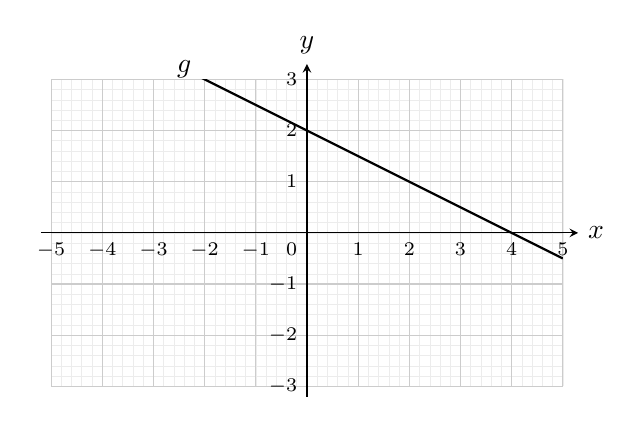
\begin{tikzpicture}[scale=0.65,>=stealth]
        % Raster
        \draw[step=0.2,gray!15,very thin]
        (-5,-3) grid (5,3);
        \draw[step=1,gray!40,thin]
        (-5,-3) grid (5,3);

        % Achsen
        \draw[->] (-5.2,0) -- (5.3,0) node[right] {\(x\)};
        \draw[->] (0,-3.2) -- (0,3.3) node[above] {\(y\)};

        \foreach \x in {-5,...,5} {
                \ifnum\x=0\relax\else
                    \node[below,font=\scriptsize] at (\x,0) {\(\x\)};
                \fi
            }

        \foreach \y in {-3,-2,-1,1,2,3}
        \node[left,font=\scriptsize] at (0,\y) {\(\y\)};

        \node[below left,font=\scriptsize] at (0,0) {\(0\)};

        % Gerade
        \begin{scope}
            \clip (-5,-3) rectangle (5,3);
            \draw[thick] plot[domain=-5:5]
            (\x,{-0.5*\x+2});
        \end{scope}

        \node at (-2.4,3.2) {\(g\)};
    \end{tikzpicture}
\end{center}

\medskip

Speziell: Auch Geraden, die nicht Graph einer Funktion sind,
lassen sich durch eine Gleichung darstellen. Zum Beispiel
ist \(h:x=1\) die Menge aller Punkte mit der \(x\)-Koordinate
\(1\) -- also eine vertikale Gerade.

\begin{center}
    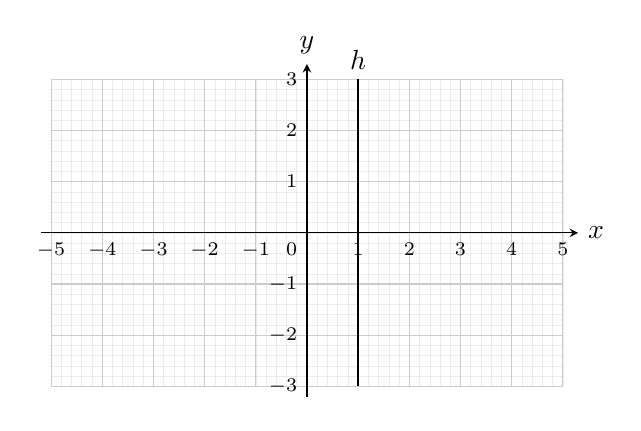
\begin{tikzpicture}[scale=0.65,>=stealth]
        % Raster
        \draw[step=0.2,gray!15,very thin]
        (-5,-3) grid (5,3);
        \draw[step=1,gray!40,thin]
        (-5,-3) grid (5,3);

        % Achsen
        \draw[->] (-5.2,0) -- (5.3,0) node[right] {\(x\)};
        \draw[->] (0,-3.2) -- (0,3.3) node[above] {\(y\)};

        \foreach \x in {-5,...,5} {
                \ifnum\x=0\relax\else
                    \node[below,font=\scriptsize] at (\x,0) {\(\x\)};
                \fi
            }

        \foreach \y in {-3,-2,-1,1,2,3}
        \node[left,font=\scriptsize] at (0,\y) {\(\y\)};

        \node[below left,font=\scriptsize] at (0,0) {\(0\)};

        % Vertikale Gerade
        \draw[thick] (1,-3) -- (1,3);
        \node[above] at (1,3) {\(h\)};
    \end{tikzpicture}
\end{center}

Durch diese Übersetzung von Punkten und Geraden in
algebraische Objekte lassen sich geometrische Fragestellungen
mit algebraischen Methoden lösen.

\textbf{Streckenlängen:} Sind zwei Punkte durch ihre Koordinaten gegeben, kann man die Länge
der Verbindungsstrecke mit Pythagoras berechnen.

Für \(A=(-2|1)\) und \(B=(3|-2)\) gilt:
\[
    \overline{AB}
    =\sqrt{(\Delta x)^2+(\Delta y)^2}
    =\sqrt{5^2+3^2}
    =\sqrt{34}.
\]

\begin{center}
    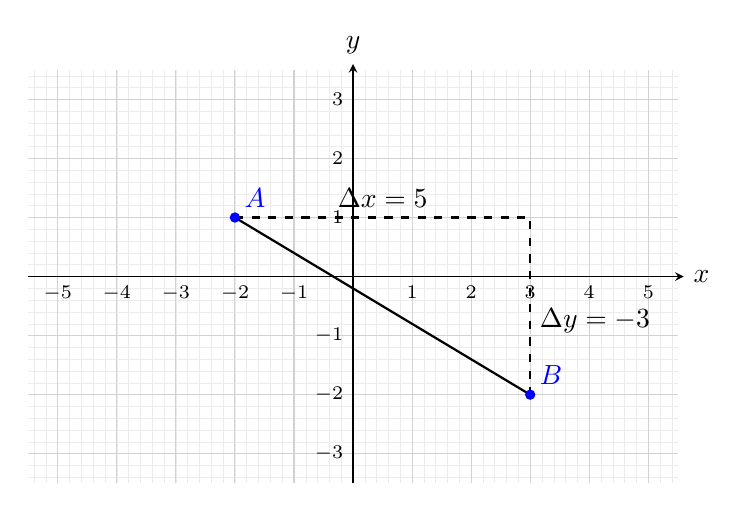
\begin{tikzpicture}[scale=0.75,>=stealth]
        % Raster
        \draw[step=0.2,gray!15,very thin]
        (-5.5,-3.5) grid (5.5,3.5);
        \draw[step=1,gray!35,thin]
        (-5.5,-3.5) grid (5.5,3.5);

        % Achsen
        \draw[->] (-5.5,0) -- (5.6,0) node[right] {\(x\)};
        \draw[->] (0,-3.5) -- (0,3.6) node[above] {\(y\)};

        \foreach \x in {-5,-4,-3,-2,-1,1,2,3,4,5}
        \node[below,font=\scriptsize] at (\x,0) {\(\x\)};
        \foreach \y in {-3,-2,-1,1,2,3}
        \node[left,font=\scriptsize] at (0,\y) {\(\y\)};

        % Verbindungsstrecke und rechtwinkliges Dreieck
        \draw[thick] (-2,1) -- (3,-2);
        \draw[dashed,thick] (-2,1) -- (3,1) -- (3,-2);

        % Punkte
        \fill[blue] (-2,1) circle (2.5pt);
        \fill[blue] (3,-2) circle (2.5pt);

        \node[blue,above right] at (-2,1) {\(A\)};
        \node[blue,above right] at (3,-2) {\(B\)};

        \node[above] at (0.5,1) {\(\Delta x=5\)};
        \node[right] at (3,-0.75) {\(\Delta y=-3\)};
    \end{tikzpicture}
\end{center}


\textbf{Schnittpunkt:} Zwei Geraden seien durch ihre Gleichungen gegeben:
\[
    g:\ y=-\frac12 x+2
    \qquad\text{und}\qquad
    k:\ y=2x-\frac13.
\]

\begin{center}
    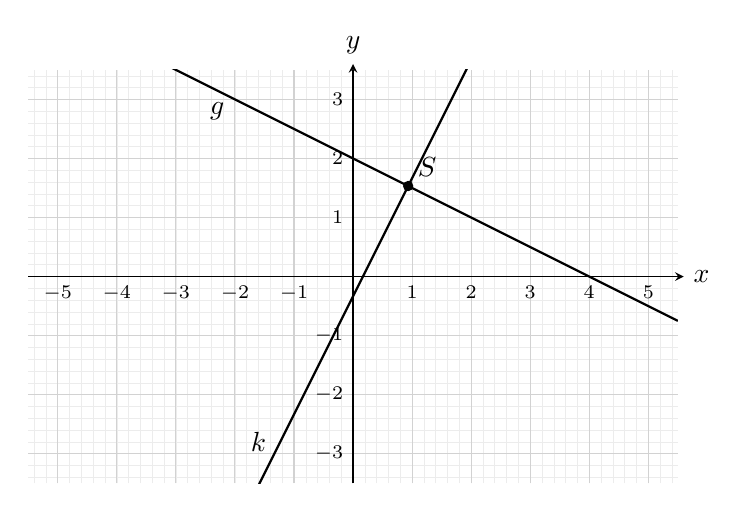
\begin{tikzpicture}[scale=0.75,>=stealth]
        % Raster
        \draw[step=0.2,gray!15,very thin]
        (-5.5,-3.5) grid (5.5,3.5);
        \draw[step=1,gray!35,thin]
        (-5.5,-3.5) grid (5.5,3.5);

        % Achsen
        \draw[->] (-5.5,0) -- (5.6,0) node[right] {\(x\)};
        \draw[->] (0,-3.5) -- (0,3.6) node[above] {\(y\)};

        \foreach \x in {-5,-4,-3,-2,-1,1,2,3,4,5}
        \node[below,font=\scriptsize] at (\x,0) {\(\x\)};
        \foreach \y in {-3,-2,-1,1,2,3}
        \node[left,font=\scriptsize] at (0,\y) {\(\y\)};

        % Geraden
        \begin{scope}
            \clip (-5.5,-3.5) rectangle (5.5,3.5);
            \draw[thick,domain=-5.5:5.5]
            plot (\x,{-0.5*\x+2});
            \draw[thick,domain=-5.5:5.5]
            plot (\x,{2*\x-1/3});
        \end{scope}

        % Schnittpunkt
        \fill (14/15,23/15) circle (2.5pt);
        \node[above right] at (14/15,23/15) {\(S\)};

        \node at (-2.3,2.8) {\(g\)};
        \node at (-1.6,-2.8) {\(k\)};
    \end{tikzpicture}
\end{center}

Die Koordinaten \((x_S|y_S)\) des Schnittpunktes \(S\)
lassen sich auf algebraische Weise bestimmen.

\(S\) liegt auf der Geraden \(g\). Das ist genau dann der Fall, wenn
\[
    y_S=-\frac12 x_S+2.
\]

\(S\) liegt auf der Geraden \(k\). Das ist genau dann der Fall, wenn
\[
    y_S=2x_S-\frac13.
\]

Daraus folgt die Gleichung:
\begin{align*}
    -\frac12 x_S+2 & = 2x_S-\frac13
                   &                  & \mid\cdot 6 \\
    -3x_S+12       & = 12x_S-2
                   &                  & \mid+3x_S+2 \\
    14             & = 15x_S
                   &                  & \mid:\,15   \\
    x_S            & = \frac{14}{15}.
\end{align*}

Die \(y\)-Koordinate des Schnittpunktes kann berechnet werden,
indem man die \(x\)-Koordinate in eine der Geradengleichungen einsetzt:
\[
    y_S=-\frac12\cdot\frac{14}{15}+2
    =\frac{23}{15}.
\]

Damit ist
\[
    \boxed{S=\left(\frac{14}{15}\,\middle|\,\frac{23}{15}\right)}.
\]


\textbf{Parallele Geraden:} Zwei Geraden
\[
    g:\ y=a_1x+b_1
    \qquad\text{und}\qquad
    p:\ y=a_2x+b_2
\]
sind genau dann parallel, wenn ihre beiden Steigungen gleich sind:
\[
    \boxed{a_1=a_2}.
\]

Auch zwei vertikale Geraden sind parallel.

In der folgenden Skizze haben beide Geraden die Steigung
\(a=-\frac12\).

\begin{center}
    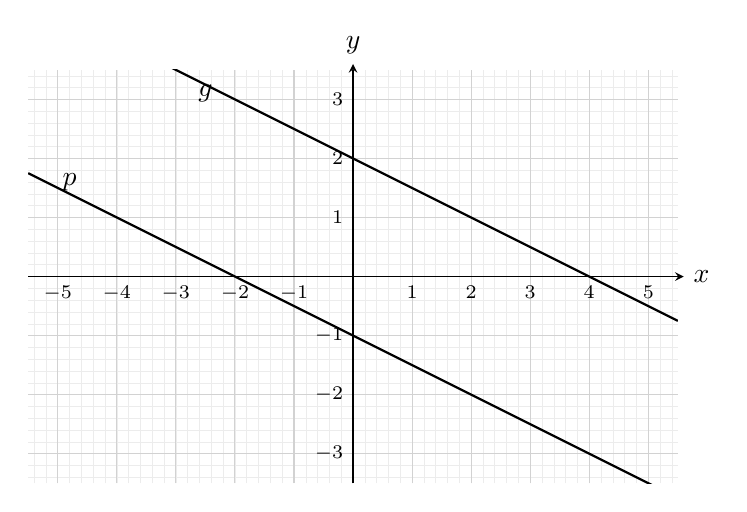
\begin{tikzpicture}[scale=0.75,>=stealth]
        % Raster
        \draw[step=0.2,gray!15,very thin]
        (-5.5,-3.5) grid (5.5,3.5);
        \draw[step=1,gray!35,thin]
        (-5.5,-3.5) grid (5.5,3.5);

        % Achsen
        \draw[->] (-5.5,0) -- (5.6,0) node[right] {\(x\)};
        \draw[->] (0,-3.5) -- (0,3.6) node[above] {\(y\)};

        \foreach \x in {-5,-4,-3,-2,-1,1,2,3,4,5}
        \node[below,font=\scriptsize] at (\x,0) {\(\x\)};
        \foreach \y in {-3,-2,-1,1,2,3}
        \node[left,font=\scriptsize] at (0,\y) {\(\y\)};

        % Parallele Geraden
        \begin{scope}
            \clip (-5.5,-3.5) rectangle (5.5,3.5);
            \draw[thick,domain=-5.5:5.5]
            plot (\x,{-0.5*\x+2});
            \draw[thick,domain=-5.5:5.5]
            plot (\x,{-0.5*\x-1});
        \end{scope}

        \node at (-2.5,3.1) {\(g\)};
        \node at (-4.8,1.6) {\(p\)};
    \end{tikzpicture}
\end{center}


\textbf{Senkrechte Geraden:}
Wie erkennt man anhand der Gleichungen, ob zwei Geraden
senkrecht verlaufen?

Dazu überlegt man sich am besten, was mit der Steigung
geschieht, wenn eine Gerade \(g\) um \(90^\circ\) gedreht wird.

\begin{center}
    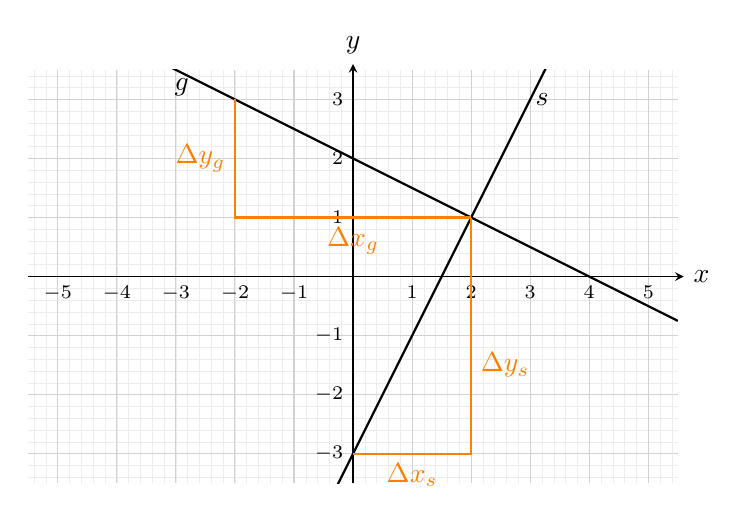
\begin{tikzpicture}[scale=0.75,>=stealth]
        % Raster
        \draw[step=0.2,gray!15,very thin]
        (-5.5,-3.5) grid (5.5,3.5);
        \draw[step=1,gray!35,thin]
        (-5.5,-3.5) grid (5.5,3.5);

        % Achsen
        \draw[->] (-5.5,0) -- (5.6,0) node[right] {\(x\)};
        \draw[->] (0,-3.5) -- (0,3.6) node[above] {\(y\)};

        \foreach \x in {-5,-4,-3,-2,-1,1,2,3,4,5}
        \node[below,font=\scriptsize] at (\x,0) {\(\x\)};
        \foreach \y in {-3,-2,-1,1,2,3}
        \node[left,font=\scriptsize] at (0,\y) {\(\y\)};

        % Geraden
        \begin{scope}
            \clip (-5.5,-3.5) rectangle (5.5,3.5);
            \draw[thick,domain=-5.5:5.5]
            plot (\x,{-0.5*\x+2});
            \draw[thick,domain=-5.5:5.5]
            plot (\x,{2*\x-3});
        \end{scope}

        % Steigungsdreieck für g
        \draw[orange,thick]
        (-2,3) -- (-2,1) -- (2,1);
        \node[orange,left] at (-2,2) {\(\Delta y_g\)};
        \node[orange,below] at (0,1) {\(\Delta x_g\)};

        % Steigungsdreieck für s
        \draw[orange,thick]
        (0, -3) -- (2,-3) -- (2,1) ;
        \node[orange,right] at (2,-1.5) {\(\Delta y_s\)};
        \node[orange,below] at (1,-3) {\(\Delta x_s\)};

        \node at (-2.9,3.2) {\(g\)};
        \node at (3.2,3) {\(s\)};
    \end{tikzpicture}
\end{center}

In der Skizze erkennt man, dass aus «vorwärts» «obsi»
wird und aus «nidsi» «vorwärts».

Anders gesagt:
\[
    \Delta y_s=\Delta x_g
    \qquad\text{und}\qquad
    \Delta x_s=-\Delta y_g.
\]

Für die Steigung der Senkrechten gilt also
\[
    a_s
    =\frac{\Delta y_s}{\Delta x_s}
    =\frac{\Delta x_g}{-\Delta y_g}
    =-\frac1{a_g}
    \quad\Longleftrightarrow\quad
    \boxed{a_s\cdot a_g=-1}.
\]

\textbf{Fazit:}
Zwei Geraden sind genau dann senkrecht zueinander, wenn
das Produkt ihrer beiden Steigungen \(-1\) ergibt.

Eine horizontale und eine vertikale Gerade stehen ebenfalls
senkrecht aufeinander.






\clearpage
\begin{ueb}
    {Analytische Geometrie}{}
    \begin{enumerate}
        \item Und? Bilden die Geraden aus \Cref{LA:Quadrat?} ein Quadrat?

        \item Berechnen Sie die Koordinaten des Schnittpunktes
              der Geraden \(g\) und \(h\).

              \begin{enumerate}
                  \item \(g:\ y=\frac13 x+1,\qquad
                        h:\ y=-\frac35 x+5\)

                  \item \(g:\ y=-\frac13 x-1,\qquad
                        h:\ y=-\frac34 x+2\)
              \end{enumerate}

        \item Bestimmen Sie rechnerisch die Koordinaten
              der drei Schnittpunkte der skizzierten Geraden.

              \begin{enumerate}
                  \item
                        \begin{center}
                            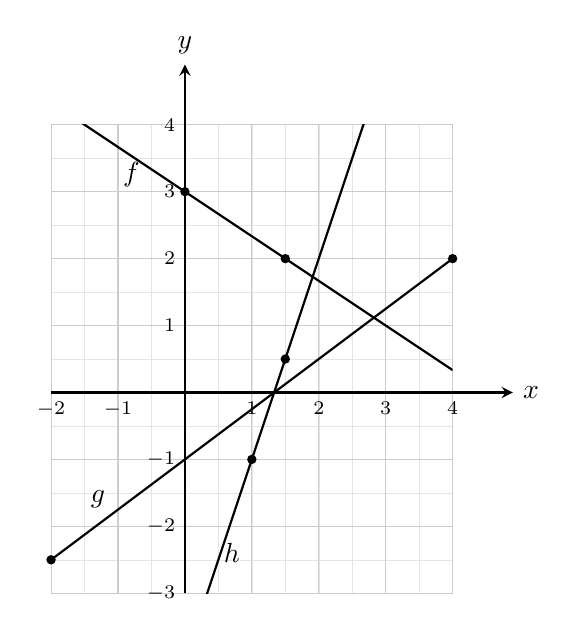
\begin{tikzpicture}[scale=0.85,>=stealth]
                                % Raster
                                \draw[step=0.5,gray!20,very thin]
                                (-2,-3) grid (4,4);
                                \draw[step=1,gray!40,thin]
                                (-2,-3) grid (4,4);

                                % Achsen
                                \draw[->,thick] (-2,0) -- (4.9,0)
                                node[right] {\(x\)};
                                \draw[->,thick] (0,-3) -- (0,4.9)
                                node[above] {\(y\)};

                                % Achsenbeschriftungen
                                \foreach \x in {-2,-1,1,2,3,4}
                                \node[below,font=\scriptsize]
                                at (\x,0) {\(\x\)};
                                \foreach \y in {-3,-2,-1,1,2,3,4}
                                \node[left,font=\scriptsize]
                                at (0,\y) {\(\y\)};

                                % Geraden
                                \begin{scope}
                                    \clip (-2,-3) rectangle (4,4);

                                    % f: y = -2/3 x + 3
                                    \draw[thick,domain=-2:4]
                                    plot (\x,{-2/3*\x+3});

                                    % g: y = 3/4 x - 1
                                    \draw[thick,domain=-2:4]
                                    plot (\x,{3/4*\x-1});

                                    % h: y = 3x - 4
                                    \draw[thick,domain=-2:4]
                                    plot (\x,{3*\x-4});
                                \end{scope}

                                % Markierte Punkte
                                \foreach \x/\y in {
                                        0/3,1.5/2,
                                        -2/-2.5,4/2,
                                        1/-1,1.5/0.5
                                    } {
                                        \fill (\x,\y) circle (2pt);
                                    }

                                % Beschriftungen
                                \node at (-0.8,3.25) {\(f\)};
                                \node at (-1.3,-1.6) {\(g\)};
                                \node at (0.7,-2.4) {\(h\)};
                            \end{tikzpicture}
                        \end{center}

                  \item
                        \begin{center}
                            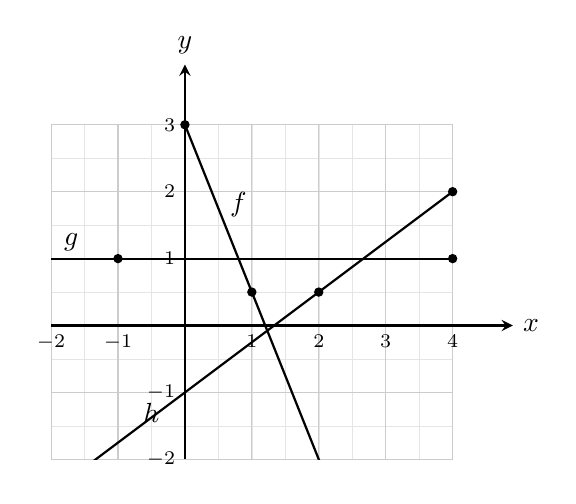
\begin{tikzpicture}[scale=0.85,>=stealth]
                                % Raster
                                \draw[step=0.5,gray!20,very thin]
                                (-2,-2) grid (4,3);
                                \draw[step=1,gray!40,thin]
                                (-2,-2) grid (4,3);

                                % Achsen
                                \draw[->,thick] (-2,0) -- (4.9,0)
                                node[right] {\(x\)};
                                \draw[->,thick] (0,-2) -- (0,3.9)
                                node[above] {\(y\)};

                                % Achsenbeschriftungen
                                \foreach \x in {-2,-1,1,2,3,4}
                                \node[below,font=\scriptsize]
                                at (\x,0) {\(\x\)};
                                \foreach \y in {-2,-1,1,2,3}
                                \node[left,font=\scriptsize]
                                at (0,\y) {\(\y\)};

                                % Geraden
                                \begin{scope}
                                    \clip (-2,-2) rectangle (4,3);

                                    % f: y = -5/2 x + 3
                                    \draw[thick,domain=-2:4]
                                    plot (\x,{-5/2*\x+3});

                                    % g: y = 1
                                    \draw[thick] (-2,1) -- (4,1);

                                    % h: y = 3/4 x - 1
                                    \draw[thick,domain=-2:4]
                                    plot (\x,{3/4*\x-1});
                                \end{scope}

                                % Markierte Punkte
                                \foreach \x/\y in {
                                        0/3,1/0.5,
                                        -1/1,4/1,
                                        2/0.5,4/2
                                    } {
                                        \fill (\x,\y) circle (2pt);
                                    }

                                % Beschriftungen
                                \node at (0.8,1.8) {\(f\)};
                                \node at (-1.7,1.25) {\(g\)};
                                \node at (-0.5,-1.3) {\(h\)};
                            \end{tikzpicture}
                        \end{center}
              \end{enumerate}
              % \item Gegeben ist die Gerade \(g\) mit der Funktionsgleichung
              %       \[
              %           g:\ y=\frac{3}{8}x-2.
              %       \]

              %       \begin{enumerate}
              %           \item Zeichnen Sie \(g\) mithilfe des \(y\)-Achsenabschnitts
              %                 und der Steigung in ein Koordinatensystem.

              %           \item Verschieben Sie \(g\) um 2 Einheiten nach links
              %                 (in negative \(x\)-Richtung) und um 3 Einheiten
              %                 nach oben (in positive \(y\)-Richtung).
              %                 Zeichnen Sie die verschobene Gerade \(g'\)
              %                 ebenfalls in dasselbe Koordinatensystem und
              %                 geben Sie die Funktionsgleichung von \(g'\) an.

              %           \item Spiegeln Sie \(g\) an der \(y\)-Achse und zeichnen
              %                 Sie die gespiegelte Gerade \(g''\) ebenfalls in
              %                 dasselbe Koordinatensystem.
              %                 Geben Sie die Gleichung von \(g''\) an.

              %           \item Zeichnen Sie zusätzlich die Gerade
              %                 \(a:\ y=-x\) ein.
              %                 Spiegeln Sie dann \(g\) an der Geraden \(a\)
              %                 und zeichnen Sie die gespiegelte Gerade
              %                 \(g'''\) ebenfalls in dasselbe Koordinatensystem.
              %                 Bestimmen Sie die Gleichung von \(g'''\).
              %       \end{enumerate}

              %       \begin{center}
              %           \begin{tikzpicture}[scale=0.7,>=stealth]
              %               % Feines Raster
              %               \draw[step=0.5,gray!20,very thin]
              %               (-8,-6) grid (8,6);

              %               % Hauptraster
              %               \draw[step=1,gray!40,thin]
              %               (-8,-6) grid (8,6);

              %               % Koordinatenachsen
              %               \draw[->,thick] (-8,0) -- (8.4,0)
              %               node[right] {\(x\)};
              %               \draw[->,thick] (0,-6) -- (0,6.4)
              %               node[above] {\(y\)};

              %               % Achsenbeschriftungen
              %               \foreach \x in {-8,-6,-4,-2,2,4,6,8}
              %               \node[below,font=\scriptsize]
              %               at (\x,0) {\(\x\)};

              %               \foreach \y in {-6,-4,-2,2,4,6}
              %               \node[left,font=\scriptsize]
              %               at (0,\y) {\(\y\)};

              %               \node[below left] at (0,0) {\(0\)};
              %           \end{tikzpicture}
              %       \end{center}

        \item Gegeben ist die Gerade \(g\) mit der Funktionsgleichung
              \[
                  g:\ y=\frac{2}{3}x-1.
              \]
              Geben Sie die Gleichung derjenigen Geraden an, die

              \begin{enumerate}
                  \item senkrecht zu \(g\) ist und durch den Ursprung geht.

                  \item senkrecht zu \(g\) verläuft und durch
                        \(Q=(-5|2)\) geht.

                  \item im Punkt \(P=(-3|g(-3))\) senkrecht zu \(g\) ist.
              \end{enumerate}

        \item \textbf{Challenge:}
              \begin{enumerate}
                  \item Berechnen Sie den Abstand der Geraden
                        \(g:\ 4x+3y=30\) vom Ursprung.

                  \item Berechnen Sie den Abstand der beiden parallelen Geraden
                        \[
                            g:\ y=\frac43x-5
                            \qquad\text{und}\qquad
                            h:\ y=\frac43x+10.
                        \]

                  \item Berechnen Sie die Länge der Höhe \(h_a\) des Dreiecks
                        \(A=(-3|4)\), \(B=(-4|-3)\), \(C=(8|6)\).
              \end{enumerate}
    \end{enumerate}

\end{ueb}

\clearpage
\textbf{Lösungen:}
\textbf{Kurzlösungen:}

\begin{enumerate}

    \item
          Ja, es ist ein Quadrat mit Seitenlänge \(s = \sqrt{\frac{36}{5}} = \frac{6}{5} \sqrt{5}\)

    \item
          \begin{enumerate}
              \item
                    \[
                        \frac13 x+1=-\frac35 x+5
                        \quad\Longrightarrow\quad
                        \boxed{S=\left(\frac{30}{7}\middle|\frac{17}{7}\right)}
                    \]

              \item
                    \[
                        -\frac13 x-1=-\frac34 x+2
                        \quad\Longrightarrow\quad
                        \boxed{S=\left(\frac{36}{5}\middle|-\frac{17}{5}\right)}
                    \]
          \end{enumerate}

    \item
          \begin{enumerate}
              \item
                    Die Geradengleichungen lauten
                    \[
                        f(x)=-\frac23x+3,\qquad
                        g(x)=\frac34x-1,\qquad
                        h(x)=3x-4.
                    \]

                    Die Schnittpunkte sind
                    \[
                        \boxed{
                            \begin{aligned}
                                S_{fg} & =\left(\frac{48}{17}\middle|\frac{19}{17}\right), \\[2mm]
                                S_{fh} & =\left(\frac{21}{11}\middle|\frac{19}{11}\right), \\[2mm]
                                S_{gh} & =\left(\frac43\middle|0\right).
                            \end{aligned}
                        }
                    \]

              \item
                    Die Geradengleichungen lauten
                    \[
                        f(x)=-\frac52x+3,\qquad
                        g(x)=1,\qquad
                        h(x)=\frac34x-1.
                    \]

                    Die Schnittpunkte sind
                    \[
                        \boxed{
                            \begin{aligned}
                                S_{fg} & =\left(\frac45\middle|1\right),                   \\[2mm]
                                S_{fh} & =\left(\frac{16}{13}\middle|-\frac{1}{13}\right), \\[2mm]
                                S_{gh} & =\left(\frac83\middle|1\right).
                            \end{aligned}
                        }
                    \]
          \end{enumerate}

    \item
          Die Steigung jeder gesuchten Geraden beträgt
          \[
              a=-\frac32.
          \]

          \begin{enumerate}
              \item
                    \[
                        \boxed{y=-\frac32x}
                    \]

              \item
                    \[
                        2=-\frac32\cdot(-5)+b
                        \quad\Longrightarrow\quad b=-\frac{11}{2}
                    \]
                    \[
                        \boxed{y=-\frac32x-\frac{11}{2}}
                    \]

              \item
                    \[
                        g(-3)=\frac23\cdot(-3)-1=-3
                    \]
                    Also ist \(P=(-3|-3)\).
                    \[
                        -3=-\frac32\cdot(-3)+b
                        \quad\Longrightarrow\quad b=-\frac{15}{2}
                    \]
                    \[
                        \boxed{y=-\frac32x-\frac{15}{2}}
                    \]
          \end{enumerate}

    \item
          \begin{enumerate}
              \item
                    \(
                    d=6
                    \)

              \item
                    \(
                    d=9
                    \)

              \item
                    \(
                    h_a =5
                    \)
          \end{enumerate}

\end{enumerate}